%%%%%%%%%%%%%%%%%%%%%%%%%%%%%%%%%%%%%%%%%%%%%%%%%%%%%%%%%%%%%%%%%%%%%%%%%%%%%%%%%
% Seminar deck (60 minutes)
% "Hedge Fund Trading and Sovereign Bond Yield Sensitivity"
% Felix Hermes (Goethe University Frankfurt & ECB)
%
% Style: clean Goldsmith-Pinkham / BSS layout (Lato, no outer theme),
%        re-coloured to a Goethe Frankfurt deep-blue identity.
% Writing convention: no colons, semicolons, or dashes used as sentence breaks.
%%%%%%%%%%%%%%%%%%%%%%%%%%%%%%%%%%%%%%%%%%%%%%%%%%%%%%%%%%%%%%%%%%%%%%%%%%%%%%%%%

\documentclass[aspectratio=169,10pt]{beamer}
\mode<presentation>

%----------------------------------------------------------------------------------------
%	FONTS, MATH, PACKAGES
%----------------------------------------------------------------------------------------
\usepackage[T1]{fontenc}
\usepackage[default]{lato}

\usepackage{amsfonts}
\usepackage{amssymb}
\usepackage{amsmath}
\usepackage{bm}

\usepackage{pifont}
\usepackage{eurosym}
\usepackage{booktabs}
\usepackage{colortbl}
\usepackage{adjustbox}
\usepackage{tabularx}
\usepackage{array}
\usepackage{graphicx}
\usepackage{subcaption}
\usepackage{enumerate}
\usepackage[font=footnotesize,labelfont=bf]{caption}
\usepackage[absolute,overlay]{textpos}
\usepackage{tikz}
\usetikzlibrary{calc,positioning,arrows.meta,decorations.pathreplacing}
\usepackage{appendixnumberbeamer}
\usepackage[dvipsnames]{xcolor}
\usepackage{hyperref}

% Author-year citations via biblatex/biber (robust under beamer; natbib=true keeps
% the familiar \citet / \citep commands working unchanged).
\usepackage{csquotes}
\usepackage[style=authoryear,natbib=true,maxcitenames=2,uniquelist=false,
            doi=false,isbn=false,url=false,eprint=false,backend=biber]{biblatex}
\addbibresource{references.bib}
% Compact in-text citation spacing
\renewcommand*{\nameyeardelim}{\addspace}

% Resolve graphics from the project root
\graphicspath{{./}{../}}

%----------------------------------------------------------------------------------------
%	GOETHE FRANKFURT COLOUR IDENTITY
%	Deep blue primary, warm accent for emphasis, green for the favourable state.
%----------------------------------------------------------------------------------------
\definecolor{goetheblue}{RGB}{0,65,106}     % primary deep blue (matches professor's UniBlue)
\definecolor{goethelink}{RGB}{0,104,168}    % brighter blue for links
\definecolor{accentred}{RGB}{196,61,33}     % warm vermillion for emphasis
\definecolor{accentgreen}{RGB}{0,128,96}    % deep green for the relaxing state
\definecolor{dividerbg}{RGB}{233,238,244}   % light blue-grey for section dividers
\definecolor{softgrey}{RGB}{140,140,140}

% Short emphasis macros
\def\hibl{\textcolor{goetheblue}}
\def\hird{\textcolor{accentred}}
\def\higr{\textcolor{accentgreen}}
\newcommand{\myemph}[1]{\textcolor{goetheblue}{\emph{#1}}}

%----------------------------------------------------------------------------------------
%	BEAMER LOOK (no outer theme; everything below drives the clean look)
%----------------------------------------------------------------------------------------
\setbeamercolor{structure}{fg=goetheblue}
\setbeamercolor{frametitle}{fg=goetheblue}
\setbeamercolor{title}{fg=goetheblue}
\setbeamercolor{subtitle}{fg=softgrey}
\setbeamercolor{author}{fg=black}
\setbeamercolor{institute}{fg=softgrey}
\setbeamercolor{alerted text}{fg=goetheblue}
\setbeamercolor{itemize item}{fg=goetheblue}
\setbeamercolor{itemize subitem}{fg=goetheblue}
\setbeamercolor{itemize subsubitem}{fg=goetheblue}
\setbeamercolor{enumerate item}{fg=goetheblue}
\setbeamercolor{block title}{fg=white,bg=goetheblue}
\setbeamercolor{block body}{fg=black,bg=goetheblue!6}
\setbeamercolor{section in toc}{fg=goetheblue}
\setbeamercolor{button}{bg=goetheblue,fg=white}

% Bold, centered frame titles, clearly larger than body text
\setbeamerfont{frametitle}{series=\bfseries,size=\large}
\setbeamerfont{title}{series=\bfseries,size=\LARGE}

% Tighter text margins (professor's layout)
\setbeamersize{text margin left=1em,text margin right=1.5em}

\setbeamertemplate{navigation symbols}{}
\setbeamertemplate{itemize items}[square]
\setbeamertemplate{section in toc}[square]

\hypersetup{
    colorlinks=true,
    citecolor=goethelink,
    linkcolor=goethelink,
    linkbordercolor={white},
    urlcolor=goethelink
}

% Centered frame title with a full-width rule a fixed, tight gap beneath.
% The rule is placed relative to the BASELINE via TikZ, so the gap is identical on
% every slide regardless of descenders (a plain \vskip is dominated by the line depth,
% which is why nudging the skip value has almost no visible effect).
\setbeamertemplate{frametitle}{%
  \vskip0.5em%
  \begin{tikzpicture}
    \node[text width=\textwidth, align=center, inner sep=0pt] (ft)
      {\usebeamerfont{frametitle}\usebeamercolor[fg]{frametitle}\insertframetitle};
    \draw[goetheblue, line width=1pt]
      ([yshift=-0.22em]ft.base west) -- ([yshift=-0.22em]ft.base east);
  \end{tikzpicture}%
  \vskip0.6em%
}

% Footline: a full-width rule with a centered tiny bold frame number (professor's layout)
\makeatletter
\setbeamertemplate{footline}{%
  \centering
  \begin{minipage}{\dimexpr\paperwidth-\beamer@leftmargin-\beamer@rightmargin\relax}
  \centering
  {\color{goetheblue}\rule{\linewidth}{0.8pt}}\vskip2pt
  {\bfseries\tiny\insertframenumber}\par
  \end{minipage}\vskip2pt
}
\makeatother

% This deck uses no Beamer navigation (no headline, nav symbols off), so suppress the
% .nav/.snm auxiliary writes. Harmless here, and it avoids an occasional flaky-disk
% corruption of those files. Remove this block if you ever re-enable navigation.
\makeatletter
\def\bm@navext{nav}\def\bm@snmext{snm}
\let\bm@orig@writefile\@writefile
\long\def\@writefile#1#2{\def\bm@thisext{#1}%
  \ifx\bm@thisext\bm@navext\else
    \ifx\bm@thisext\bm@snmext\else
      \bm@orig@writefile{#1}{#2}%
    \fi
  \fi}
\makeatother

%----------------------------------------------------------------------------------------
%	SECTION DIVIDERS (slightly shaded slide, centered blue title between two rules)
%----------------------------------------------------------------------------------------
\newenvironment{transitionframe}{%
  \setbeamercolor{background canvas}{bg=dividerbg}%
  \begin{frame}[plain,noframenumbering]\centering\vfill}{%
  \vfill\end{frame}}

\newcommand{\sectionframe}[1]{%
  \section{#1}%
  \begin{transitionframe}%
  \begin{tikzpicture}
    \node[inner sep=0pt] (st) {\LARGE\color{goetheblue}\textbf{#1}};
    % Rules placed symmetrically around the actual text box, so the title sits
    % optically centred between them whatever its ascenders/descenders.
    \draw[goetheblue, line width=1pt]
      ([xshift=-0.275\textwidth, yshift=0.85em]st.north) -- ([xshift=0.275\textwidth, yshift=0.85em]st.north);
    \draw[goetheblue, line width=1pt]
      ([xshift=-0.275\textwidth, yshift=-0.85em]st.south) -- ([xshift=0.275\textwidth, yshift=-0.85em]st.south);
  \end{tikzpicture}%
  \end{transitionframe}}

% Inner divider for the four numbered results (also shaded)
\newcommand{\resultdivider}[2]{%
  \begin{transitionframe}%
   {\large\color{goetheblue}\textbf{Finding #1}}\\[0.7em]%
   {\LARGE #2}\\[0.9em]%
   {\color{goetheblue}\rule{0.30\textwidth}{1pt}}%
  \end{transitionframe}}

%----------------------------------------------------------------------------------------
%	HELPERS
%----------------------------------------------------------------------------------------
\newcommand{\lvs}{\vspace{0.32cm}}
\newcommand{\svs}{\vspace{0.18cm}}
\newcommand{\hvs}{\vspace{0.6cm}}

\newcommand{\bit}{\begin{itemize}}
\newcommand{\eit}{\end{itemize}}
\newcommand{\ben}{\begin{enumerate}}
\newcommand{\een}{\end{enumerate}}
\newcommand{\beq}{\begin{equation*}}
\newcommand{\eeq}{\end{equation*}}

% Roomier itemize for body slides
\newenvironment{wideitemize}{\itemize\addtolength{\itemsep}{0.45pc}}{\enditemize}

% Takeaway: a filled triangle bullet with bold blue text (professor's conclusion style).
% The hanging indent keeps wrapped lines aligned under the text, not under the marker.
\newcommand{\takeaway}[1]{%
  \par\smallskip\noindent
  \hangindent=1.4em\hangafter=1
  \textcolor{goetheblue}{$\blacktriangleright$}\ {\color{goetheblue}\bfseries #1}\par}

% Bold lead-in header that stands on its own line (avoids the colon construction)
\newcommand{\lead}[1]{{\bfseries #1}\par\nopagebreak}

% ---- Table/figure notes that match the width of the object above them ---------------
% Wrap a table or figure so the following \fignote spans exactly the same width and no
% more. Two wrappers record the fractions [lf,rf] of the box that the note should span:
%   \measurebox{<obj>}          note spans the whole box (tables, lf=0, rf=1)
%   \measureplot{lf}{rf}{<fig>} note spans only the plotting area between the axes, since
%                               a plot image is padded on the left by its y-axis label and
%                               tick labels; lf,rf are the axis positions as fractions of
%                               the image width (measured once per figure).
% The note itself is set as justified block text, centered under the object. A \fignote
% with no preceding wrapper falls back to the full text width (side-by-side panel slides).
\newsavebox{\tfigbox}
\newlength{\tfigwidth}
\newlength{\tfignl}
\newlength{\tfignr}
\newif\iftfigwidth
\def\tfiglf{0}\def\tfigrf{1}
\newcommand{\measurebox}[1]{%
  \gdef\tfiglf{0}\gdef\tfigrf{1}%
  \sbox{\tfigbox}{#1}%
  \global\tfigwidth=\wd\tfigbox\relax
  \global\tfigwidthtrue
  \usebox{\tfigbox}%
}
\newcommand{\measureplot}[3]{%
  \gdef\tfiglf{#1}\gdef\tfigrf{#2}%
  \sbox{\tfigbox}{#3}%
  \global\tfigwidth=\wd\tfigbox\relax
  \global\tfigwidthtrue
  \usebox{\tfigbox}%
}

% Small grey note, leaves the bottom-right corner free for a button. Fixed gap ABOVE and
% BELOW, independent of the surrounding environment, so the note sits the same distance
% from the table and from the text on every slide. Set as justified block text in a block
% aligned to the object (full width for tables, between the axes for plots). Do not add
% \svs around it.
\newcommand{\fignote}[1]{%
  \par\addvspace{7pt}%
  \iftfigwidth
    \global\tfigwidthfalse
    \setlength{\tfignl}{\tfiglf\tfigwidth}%
    \setlength{\tfignr}{\dimexpr\tfigwidth-\tfigrf\tfigwidth\relax}%
    {\centering
     \begin{minipage}{\tfigwidth}%
       \parindent=0pt \leftskip=\tfignl \rightskip=\tfignr \emergencystretch=1.5em
       \tiny\color{softgrey} #1\par
     \end{minipage}\par}%
  \else
    {\tiny\color{softgrey} #1\par}%
  \fi
  \addvspace{9pt}%
}

% ---- Note under a two-panel figure (two images in equal 0.5\textwidth columns that fill
% the text width, each image centered in its column). Wrap the panels in \panL and \panR
% so their rendered widths are captured, then place \twopanelnote{lf}{rf}{text} after the
% columns. The note is justified block text spanning from the LEFT panel's y-axis (fraction
% lf of the left image) to the RIGHT panel's right edge (fraction rf of the right image),
% so it lines up with the plotting area exactly as the single-figure notes do.
\newlength{\panLw}\newlength{\panRw}
\newcommand{\panL}[1]{\sbox{\tfigbox}{#1}\global\panLw=\wd\tfigbox\usebox{\tfigbox}}
\newcommand{\panR}[1]{\sbox{\tfigbox}{#1}\global\panRw=\wd\tfigbox\usebox{\tfigbox}}
\newcommand{\twopanelnote}[3]{%
  \par\addvspace{7pt}%
  \setlength{\tfignl}{0.5\textwidth}\addtolength{\tfignl}{-\panLw}%   colw-panLw
  \setlength{\tfignl}{0.5\tfignl}\addtolength{\tfignl}{#1\panLw}%     (colw-panLw)/2 + lf*panLw
  \setlength{\tfignr}{0.5\textwidth}\addtolength{\tfignr}{-\panRw}%   colw-panRw
  \setlength{\tfignr}{0.5\tfignr}\addtolength{\tfignr}{\panRw}\addtolength{\tfignr}{-#2\panRw}% +(1-rf)panRw
  {\centering
   \begin{minipage}{\textwidth}%
     \parindent=0pt \leftskip=\tfignl \rightskip=\tfignr \emergencystretch=1.5em
     \tiny\color{softgrey} #3\par
   \end{minipage}\par}%
  \addvspace{9pt}%
}

% Navigation button at a fixed bottom-right position (decoupled from content flow, so it
% never collides with the body or the footer). Its right edge is aligned with the right
% end of the blue footline rule. That rule is centered inside a block of width
% \paperwidth-\beamer@leftmargin-\beamer@rightmargin, so its right end is inset from the
% page edge by half the sum of the text margins; we reuse the same inset here.
\makeatletter
\newlength{\navbtnx}
\setlength{\navbtnx}{\dimexpr\paperwidth-0.5\beamer@leftmargin-0.5\beamer@rightmargin-4cm\relax}
\makeatother
\newcommand{\navbtn}[2]{%
  \begin{textblock*}{4cm}(\navbtnx,0.915\paperheight)%
    \raggedleft\hyperlink{#1}{\beamerbutton{#2}}%
  \end{textblock*}}

% Highlight box for a headline statistic
\tikzset{keybox/.style={rectangle, rounded corners=3pt, draw=goetheblue,
  fill=goetheblue!7, line width=1pt, inner sep=8pt, align=center}}
\tikzset{redbox/.style={rectangle, rounded corners=3pt, draw=accentred,
  fill=accentred!7, line width=1pt, inner sep=6pt, align=center, font=\footnotesize}}
\tikzset{greenbox/.style={rectangle, rounded corners=3pt, draw=accentgreen,
  fill=accentgreen!7, line width=1pt, inner sep=6pt, align=center, font=\footnotesize}}
\tikzset{greybox/.style={rectangle, rounded corners=3pt, draw=black!40,
  fill=black!4, line width=0.8pt, inner sep=6pt, align=center, font=\footnotesize}}

\newcommand{\stat}[2]{\tikz[baseline]{\node[keybox]{{\large\textbf{\color{goetheblue}#1}}\\[1pt]{\footnotesize #2}};}}

% Dashed placeholder box for walkthrough figures not yet made. #1 optional width
% fraction (default 0.6), #2 a short description of the figure that will go here.
\newcommand{\figph}[2][0.6]{%
  \begin{tikzpicture}
    \node[draw=softgrey, dashed, line width=0.9pt, rounded corners=4pt,
          fill=black!2, inner sep=12pt, align=center,
          text width=#1\textwidth, minimum height=0.5\textheight]
      {{\color{softgrey}\itshape figure to come}\\[6pt]{\color{softgrey}\footnotesize #2}};
  \end{tikzpicture}}

%----------------------------------------------------------------------------------------
%	TITLE METADATA
%----------------------------------------------------------------------------------------
\title[Hedge Funds and Sovereign Bond Sensitivity]{Hedge Fund Trading and \\ Sovereign Bond Yield Sensitivity}
\author[Felix Hermes]{Felix Hermes\inst{1,2}}
\institute[]{\inst{1}Goethe University Frankfurt \quad \inst{2}European Central Bank}
% Edit the venue and date for your seminar below.
\date{DG-MF Seminar Series \\[2pt] \today}

\begin{document}

%========================================================================================
%	TITLE
%========================================================================================
\begin{frame}[plain,noframenumbering]
  \vfill
  \begin{center}
    {\color{goetheblue}\rule{0.16\textwidth}{2.2pt}}\\[0.9em]
    {\usebeamerfont{title}\usebeamercolor[fg]{title}\inserttitle}\\[1.9em]
    %{\color{softgrey}\large Job market paper}\\[1.4em]
    {\large\insertauthor}\\[0.5em]
    {\color{softgrey}\insertinstitute}\\[1.4em]
    {\color{softgrey}\insertdate}
  \end{center}
  \vfill
  \begin{center}
    {\scriptsize\color{softgrey} This paper should not be reported as representing the views of the European Central Bank (ECB). The views expressed are those of the author and do not necessarily reflect those of the ECB.}
  \end{center}
\end{frame}


% --- Scene setter: the growing hedge fund footprint (opens the intro) ---
\begin{frame}{Hedge funds are a growing force in government bond markets}
\lvs
\begin{columns}[c]
\begin{column}{0.63\textwidth}
\centering
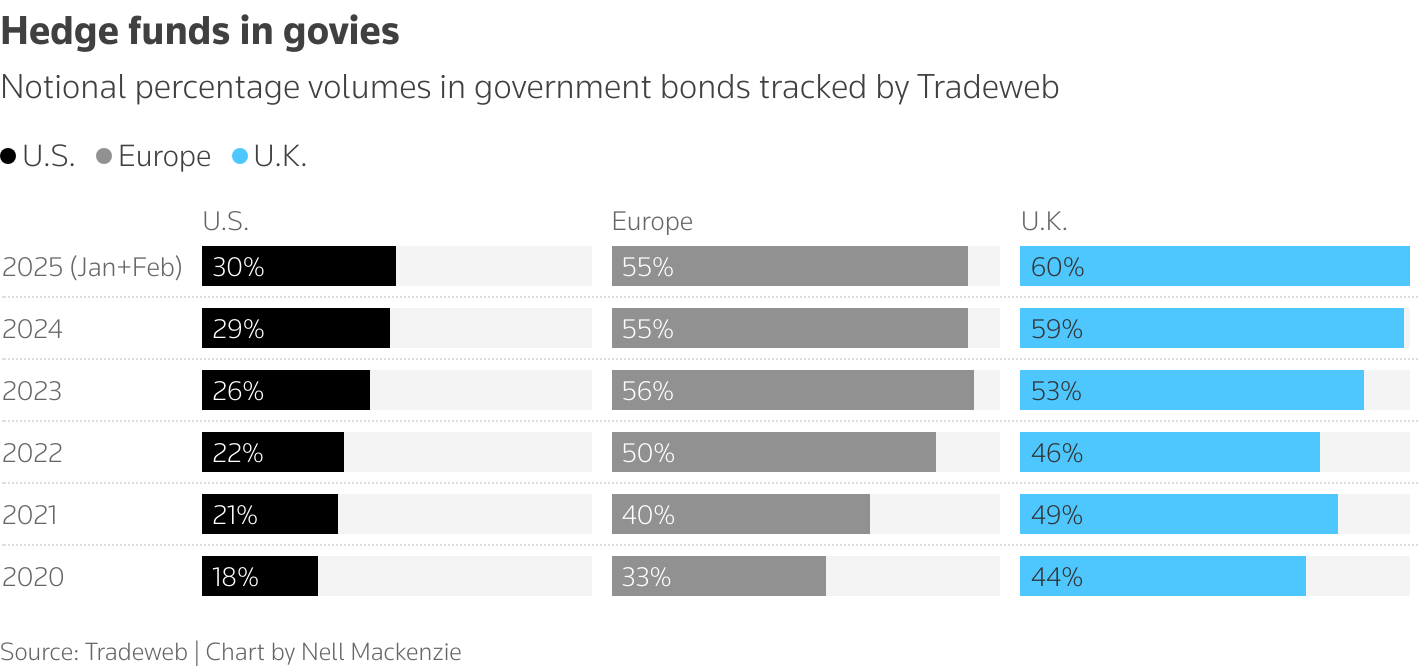
\includegraphics[width=\textwidth]{Figures/tradeweb.png}
\end{column}
\begin{column}{0.34\textwidth}
\begin{wideitemize}
  \item Their share of trading volume keeps rising since 2020
  \item In \hibl{Europe} it went from a third to \hibl{more than half} of volumes
  \item The rise is broad, across the US, Europe, and the UK
\end{wideitemize}
\end{column}
\end{columns}
\vfill
\takeaway{How does pricing change as hedge funds become more important?}
\end{frame}


% --- Two opposing views (paper intro, first paragraph) ---
\begin{frame}{Two views on the price impact of leveraged investors}
\lvs
Do hedge funds change the sensitivity of prices to shocks?
\svs
\begin{columns}[t]
\begin{column}{0.48\textwidth}
  \begin{center}
  \begin{tikzpicture}
    \node[greenbox, text width=0.9\textwidth]{%
      {\normalsize\higr{\textbf{Decrease sensitivity}}}\\[3pt]
      Their arbitrage activity corrects mispricings\\[2pt]
      Prices are pushed \emph{toward} fundamentals};
  \end{tikzpicture}\\[3pt]
  {\scriptsize\color{softgrey}\citet{gromb2002, cao2018}}
  \end{center}
\end{column}
\begin{column}{0.48\textwidth}
  \begin{center}
  \begin{tikzpicture}
    \node[redbox, text width=0.9\textwidth]{%
      {\normalsize\hird{\textbf{Increase sensitivity}}}\\[3pt]
      Leverage and funding fragility force trades\\[2pt]
      Prices are pushed \emph{away} from fundamentals};
  \end{tikzpicture}\\[3pt]
  {\scriptsize\color{softgrey}\citet{shleifer1997, brunnermeier2009, geanakoplos2010}}
  \end{center}
\end{column}
\end{columns}
\lvs
Whether hedge funds increase or decrease price sensitivity in a given situation is ultimately an empirical question, and granular evidence remains scarce.
\takeaway{This paper shows hedge funds amplify the sensitivity of sovereign bond prices to shocks}
\end{frame}

% --- Why now + the gap (second and third intro paragraphs) ---
\begin{frame}{Why this matters now}
\svs
\lead{The financial system has shifted toward nonbank intermediation}
\bit\itemsep3pt
  \item Tighter bank regulation since the global financial crisis moved activity toward nonbank financial intermediaries {\scriptsize\color{softgrey}\citep{pelizzon2025nbfi}}
  \item Offshore hedge funds stand out for their \hird{opacity} and heavy use of \hird{leverage} {\scriptsize\color{softgrey}\citep{barth2025cross, aramonte2023}}
  \item They finance positions with short term repo, which makes them sensitive to sudden moves in collateral value
\eit
\svs
\lead{The risk is procyclical amplification}
\bit\itemsep3pt
  \item Leverage can lead funds to trade with the shock rather than against it, amplifying the move instead of absorbing it
  \item March 2020 was an extreme example, when forced deleveraging by hedge funds intensified stress in the US Treasury market {\scriptsize\color{softgrey}\citep{barth2025, kruttli2025}}
\eit
\svs
\lead{What we still do not know}
\bit
  \item Whether this trading shapes pricing \hibl{outside crises}, and whether assessing the risk needs more than the presence and size of positions
\eit
\end{frame}

% --- This paper ---
\begin{frame}{This paper}
\svs
\lead{Research question}
\bit
  \item Does the leveraged positioning of hedge funds amplify sovereign bond yield sensitivity to shocks, and under what conditions?
\eit
\svs
\lead{Two ingredients the question requires}
\ben\itemsep3pt
  \item Granular positions \\
        {\footnotesize Regulatory repo data that track daily hedge fund positions in individual sovereign bonds}
  \item Clean price variation \\
        {\footnotesize High frequency monetary policy surprises that move yields exogenously {\scriptsize\color{softgrey}\citep{altavilla2019}}}
\een
\svs
\lead{Strategy}
\bit
  \item Interact \hibl{predetermined} hedge fund positions with the shock to recover the additional yield sensitivity that arises when hedge funds trade a given bond
\eit
\end{frame}

% --- Preview of the four findings ---
\begin{frame}{Four findings}
\lvs
\ben\itemsep11pt
  \item Bonds hedge funds hold are more volatile, but \hibl{only on shock days} \\
        {\footnotesize\color{softgrey} Comparable bonds are no more volatile on a normal day, so the difference is not selection}
  \item Hedge fund trading \hird{raises} the sensitivity of yields to shocks \\
        {\footnotesize\color{softgrey} Yields move further in the direction of the shock, and the move reverts within days}
  \item The effect is \hird{symmetric}, whether the shock helps or hurts the position \\
        {\footnotesize\color{softgrey} Comparable in both states, consistent with leveraged investors rebalancing toward a target}
  \item It is concentrated in \hird{directional} books \\
        {\footnotesize\color{softgrey} Carried by directional books, close to zero in hedged relative value books}
\een
\end{frame}

% --- Walkthrough 1: volatility (the baseline result) ---
\begin{frame}{Bonds hedge funds hold are more volatile, but only on shock days}
\svs
\begin{center}
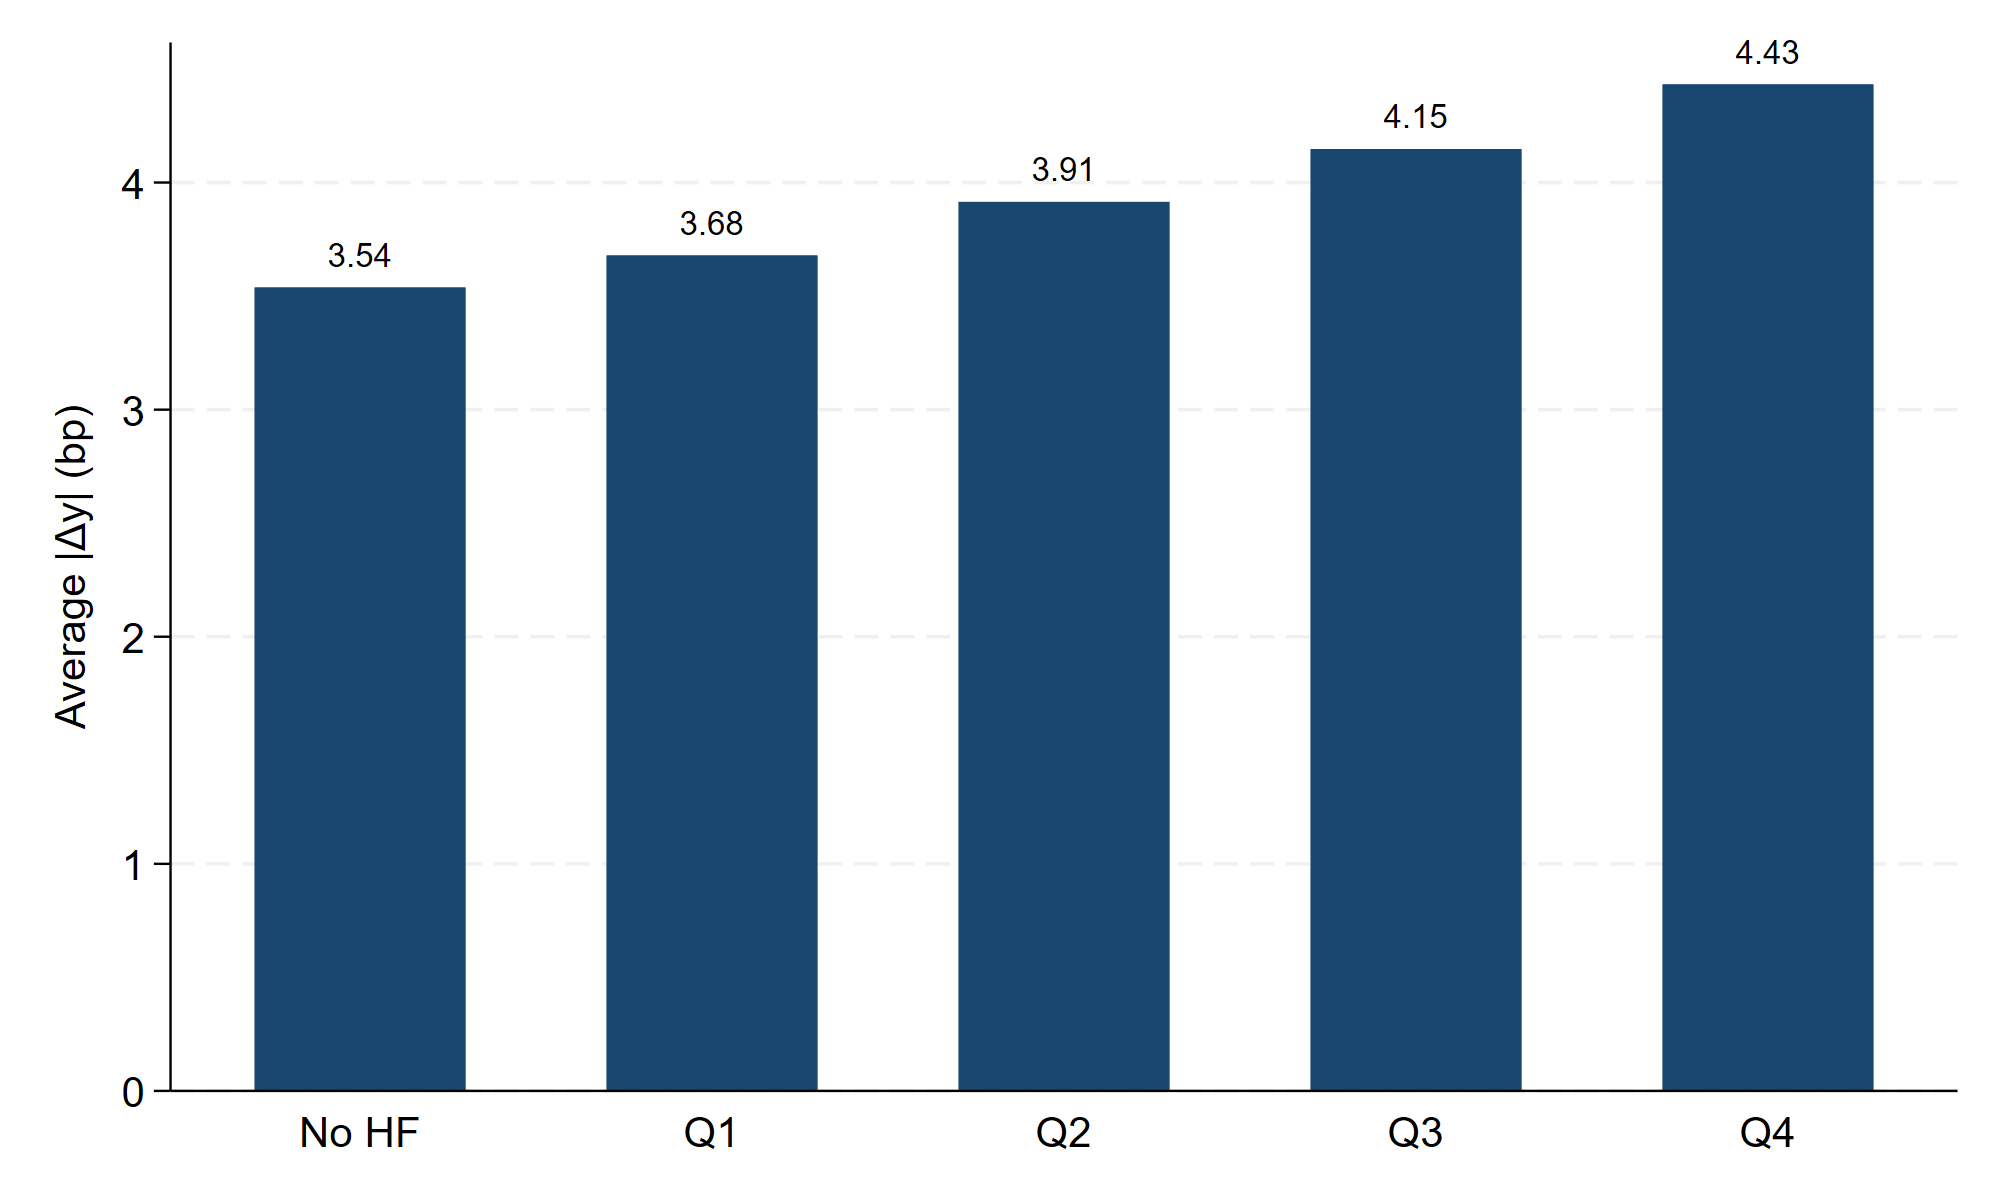
\includegraphics[width=0.72\textwidth,height=0.6\textheight,keepaspectratio]{Figures/intensity_volatility_bars.png}
\end{center}
\takeaway{It is not selection, the bonds hedge funds hold are no different on a normal day}
\end{frame}

% --- Walkthrough 2: sensitivity (scatterplot already available) ---
\begin{frame}{Hedge fund trading raises the sensitivity of yields to shocks}
\svs
\begin{center}
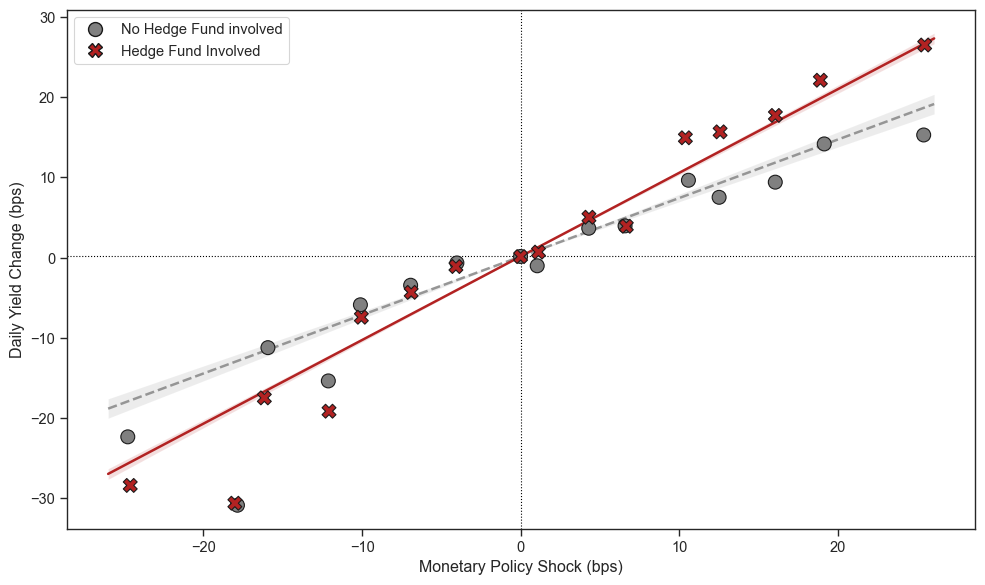
\includegraphics[width=0.72\textwidth,height=0.6\textheight,keepaspectratio]{Figures/shock_reaction_scatterplot.png}
\end{center}
\takeaway{The move is directional, and it reverts within days, a temporary dislocation}
\end{frame}

% --- Walkthrough 3: symmetry ---
\begin{frame}{The effect is symmetric, whether the shock helps or hurts the position}
\svs
\begin{center}
\figph{impulse response of the yield to a shock, constraining regime versus relaxing regime. Comparable amplification in both}
\end{center}
\takeaway{Consistent with rebalancing toward a target, not only a crisis phenomenon}
\end{frame}

% --- Walkthrough 4: directionality ---
\begin{frame}{It is concentrated in directional books}
\svs
\begin{center}
\figph{impulse response of the yield to a shock, bonds in directional books versus hedged books. Overshoot only for directional books}
\end{center}
\takeaway{So the directionality of the book matters, beyond how much hedge funds hold}
\end{frame}

% --- Related literature ---
\begin{frame}{Related literature}
\lvs
\begin{wideitemize}
  \item \textbf{Determinants of sovereign yields and non fundamental pricing}\\
        I document a specific source of temporary deviations from fundamentals\\
        {\scriptsize\color{softgrey} \citet{degauwe2013}; \citet{greenwood2014}; \citet{koijen2021}; \citet{duffie2010}}
  \item \textbf{Nonbanks and hedge funds in financial markets}\\
        I show an amplification channel that is not confined to stress episodes\\
        {\scriptsize\color{softgrey} \citet{barth2025}; \citet{kruttli2025}; \citet{anaya2025}; \citet{pelizzon2025}}
  \item \textbf{How leveraged investors transmit shocks}\\
        I show comparable amplification in the constraining and the relaxing state\\
        {\scriptsize\color{softgrey} \citet{adrian2014}; \citet{brunnermeier2009}; \citet{avalos2023}; \citet{deLong1990}; \citet{moskowitz2012}}
\end{wideitemize}
\end{frame}

%========================================================================================
\sectionframe{Data}
%========================================================================================

\begin{frame}{Data}
\svs
\lead{Hedge fund repo positions \quad {\normalfont\color{softgrey} ECB SFTDS}}
\bit\itemsep2pt
  \item Regulatory transaction data covering euro area repo activity at the transaction level
  \item Offshore hedge funds identified by Cayman Islands domicile, refined with the classification of \citet{lenoci2021}, giving \hibl{152 funds}
\eit
\svs
\lead{Bond characteristics \quad {\normalfont\color{softgrey} Bloomberg}}
\bit\itemsep2pt
  \item Daily yields, duration, bid ask spread, amount issued
  \item Cheapest to deliver status built from Eurex delivery outcomes {\scriptsize\color{softgrey}\citep{pelizzon2025}}
\eit
\svs
\lead{Exogenous shocks \quad {\normalfont\color{softgrey} EA-MPD} {\scriptsize\color{softgrey}\citep{altavilla2019}}}
\bit\itemsep2pt
  \item Intraday change in the 2 year OIS rate during the ECB monetary event window
  \item The same shock hits every bond, so identification comes from cross sectional differences in positioning
\eit
\svs
\lead{Sample}
\bit
  \item German and Italian sovereign bonds, Jan 2021 to Nov 2025 {\footnotesize\color{softgrey}(about 70\% of euro area hedge fund sovereign activity)}
\eit
\end{frame}

\begin{frame}{Hedge funds hold large, leveraged positions}
\hypertarget{footprint}{}
\lvs
\begin{columns}[c]
\begin{column}{0.5\textwidth}
\centering
\scriptsize
\setlength{\tabcolsep}{5pt}
\renewcommand{\arraystretch}{1.25}
\measurebox{\begin{tabular}{lcc}
\toprule
 & Mean & Median \\
\midrule
\multicolumn{3}{l}{\textit{Footprint}}\\
HF present (share of bond days) & 0.53 & 1.00 \\
Net position when active (\% issued) & 3.01 & 1.80 \\
\addlinespace
\multicolumn{3}{l}{\textit{Leverage and funding}}\\
Haircut, long (\%) & 0.24 & 0.12 \\
Haircut, short (\%) & $-0.08$ & $-0.05$ \\
Maturity, long (days) & 16.5 & 11.0 \\
\addlinespace
\multicolumn{3}{l}{\textit{Shock days}}\\
Tightening surprise (bps) & 5.87 & 4.95 \\
Easing surprise (bps) & $-4.17$ & $-3.13$ \\
\bottomrule
\end{tabular}}
\par\smallskip
\fignote{Daily panel of German and Italian sovereign bonds. Footprint figures are conditional on active hedge fund participation. Haircuts and maturities use active transactions. Sample period 2021 to 2025.}
\end{column}
\begin{column}{0.47\textwidth}
\begin{wideitemize}
  \item Hedge funds are active on \hibl{53\%} of bond days
  \item When active they hold \hibl{3\%} of the bond on average, an economically meaningful share
  \item Haircuts near \hibl{zero} implying high potential levels of leverage on these safe assets
  \item A typical surprise of about \hibl{4--6 bps} is enough to move a position materially
\end{wideitemize}
\end{column}
\end{columns}
\navbtn{summ_full}{Full table}
\end{frame}

%========================================================================================
\sectionframe{Stylized Facts}
%========================================================================================

% Verbal cues:
% pre-hike = carry trade (long Italy, short Germany); hike = directional, short both;
% pivot to cuts = back to carry. Positioning is dynamic, direction matters.
\begin{frame}{Hedge fund positioning rotates with the policy cycle}
\begin{center}
\measureplot{0.062}{0.991}{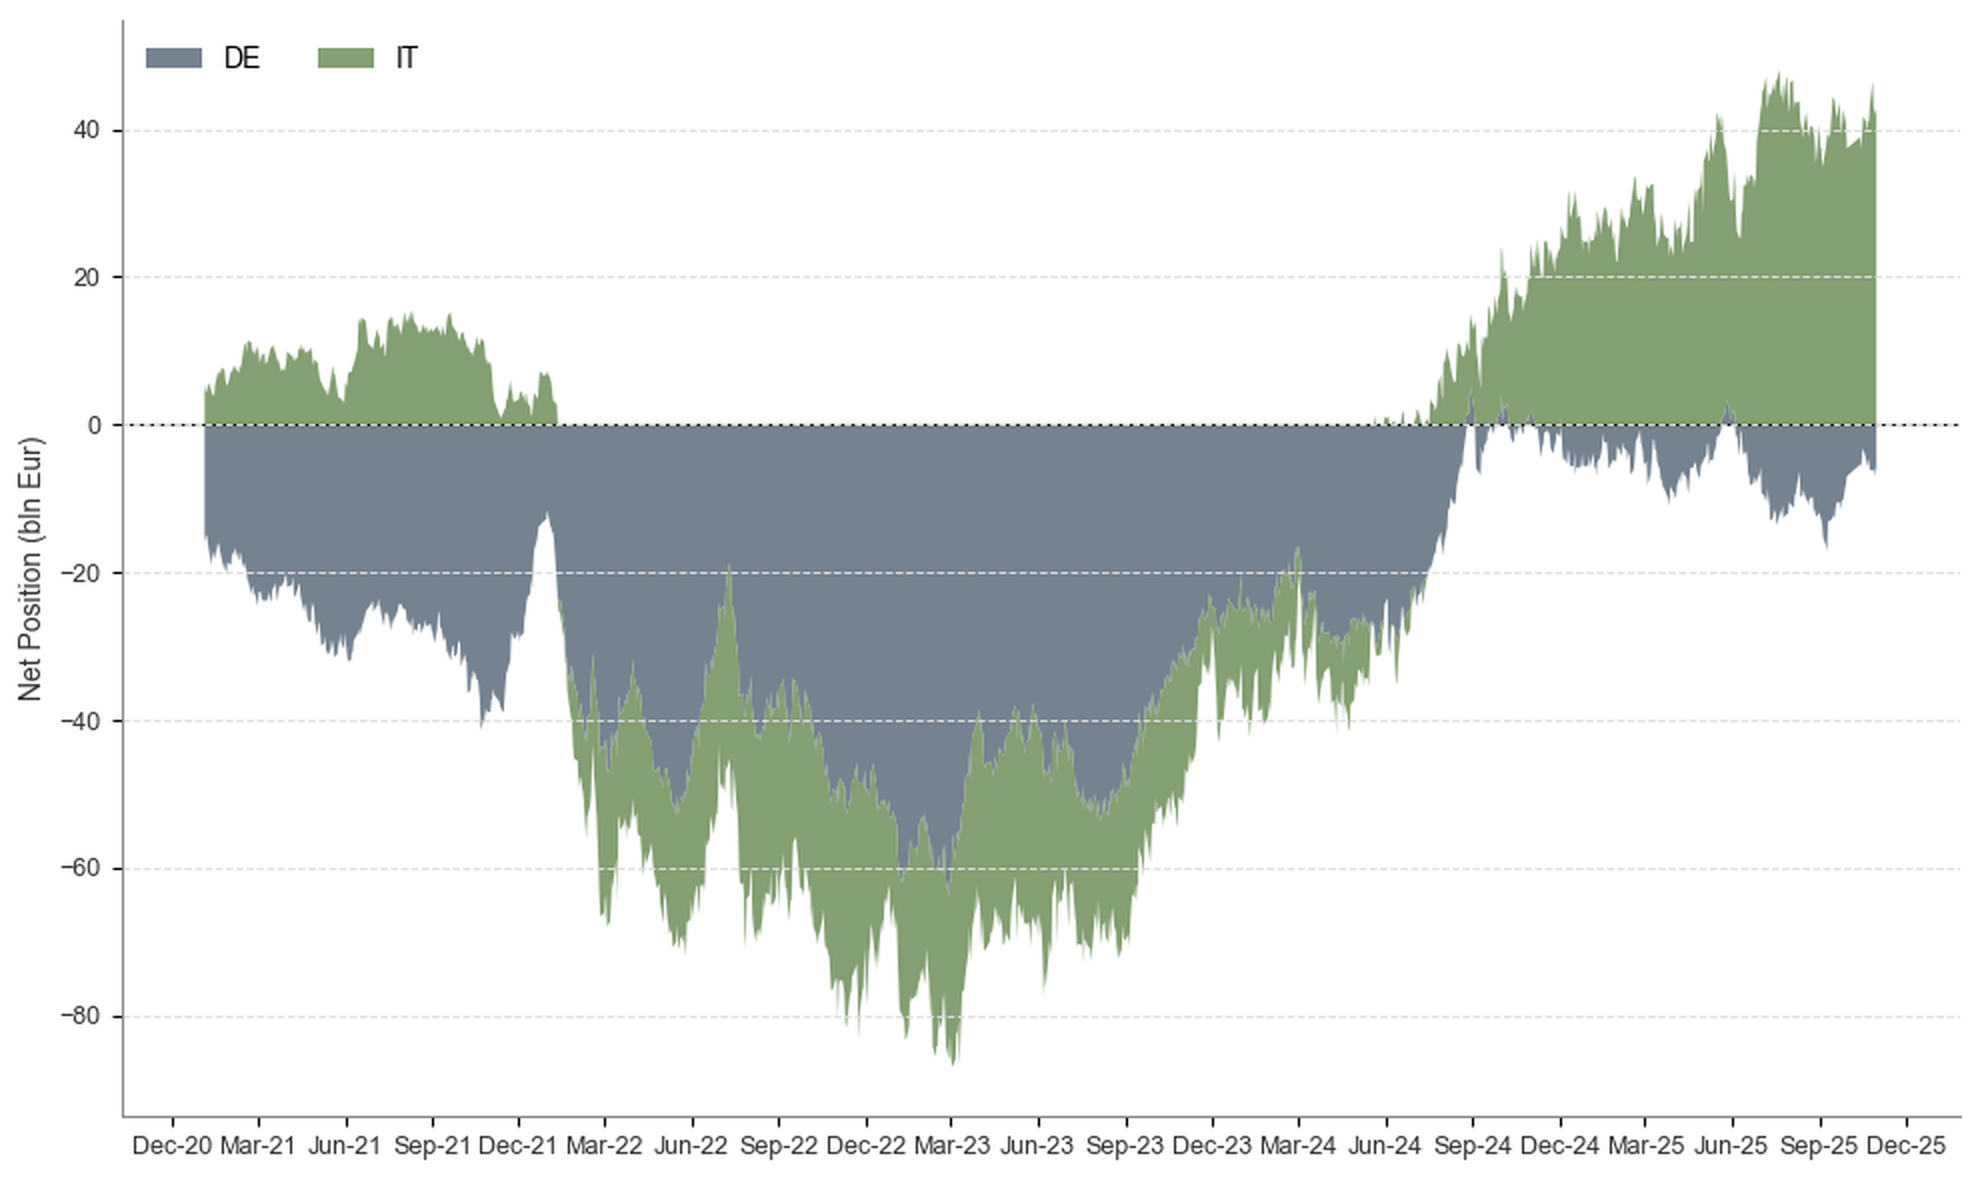
\includegraphics[height=0.72\textheight,keepaspectratio]{Figures/motivation_chart.png}}
\end{center}
\fignote{Aggregate net repo positions of offshore hedge funds in German and Italian sovereign bonds, EUR outstanding. Positive values are net cash borrowing (a proxy for long), negative values net cash lending (a proxy for short). Sample period 2021 to 2025.}
\end{frame}

% Verbal cues:
% non-HF bonds: roughly one-to-one; HF bonds steeper on both sides;
% at zero shock no difference -> presence alone does not move yields.
\begin{frame}{Yields move more on shock days when hedge funds are active}
\begin{center}
\measureplot{0.067}{0.972}{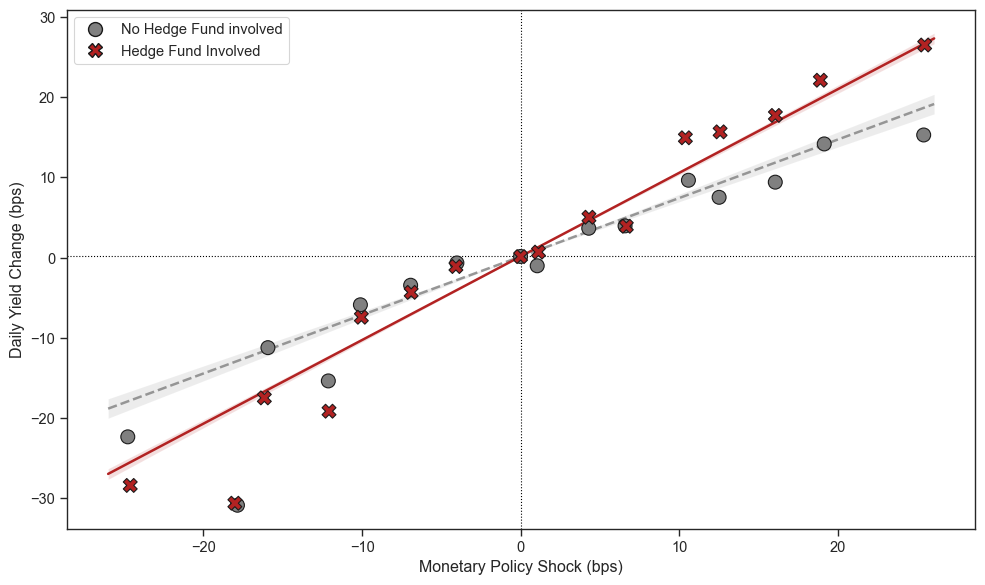
\includegraphics[width=0.76\textwidth,height=0.66\textheight,keepaspectratio]{Figures/shock_reaction_scatterplot.png}}
\end{center}
\fignote{Binned scatterplot of daily yield changes against monetary policy shocks, separately for bonds with and without active hedge fund positions. Yield changes are residualized for bond fixed effects. Lines are linear fits on the bond level data. Sample period 2021 to 2025.}
\end{frame}

%========================================================================================
\sectionframe{Mechanism}
%========================================================================================

\begin{frame}{How leveraged positioning amplifies yields}
\svs
\lead{Starting point \quad {\normalfont\color{softgrey}\citet{adrian2014}}}
\bit\itemsep1pt
  \item Leveraged intermediaries actively manage their balance sheet against the risk environment
  \item The same rule produces \hibl{opposite} position adjustments depending on the sign of the shock
\eit
\svs
\begin{center}
\scalebox{0.86}{%
\begin{tikzpicture}[font=\footnotesize,>=Stealth, node distance=3mm]
  \node[keybox, text width=4.1cm] (shock) {Shock interacts with a predetermined leveraged position};
  \node[redbox, text width=4.2cm, below left=5mm and 0.05cm of shock] (con)
    {\hird{\textbf{Constraining}}\\ price moves \emph{against} the position\\ capital buffer erodes\\ fund \hird{reduces} exposure};
  \node[greenbox, text width=4.2cm, below right=5mm and 0.05cm of shock] (rel)
    {\higr{\textbf{Relaxing}}\\ price moves \emph{in favor}\\ constraint loosens\\ fund \higr{expands} exposure};
  \draw[->,line width=0.9pt] (shock) -- (con);
  \draw[->,line width=0.9pt] (shock) -- (rel);
\end{tikzpicture}}
\end{center}
\takeaway{In both states the resulting trading pushes yields further in the direction of the initial shock}
\end{frame}

\begin{frame}{A numerical example}
\setlength\abovedisplayskip{4pt}\setlength\belowdisplayskip{4pt}
\svs
\lead{Setup \quad {\normalfont\color{softgrey} representative sample values}}
\bit\footnotesize\itemsep1pt
  \item A bond of duration about 7 years financed via repo, effective margin $m_i = 2\%$ {\scriptsize(raw haircuts 0.24\%)}
  \item Hedge funds hold $Q_{HF}/Q_{Total} = 3\%$ of the bond
  \item Tightening surprise of 6 bps, market elasticity $\lambda = 5$ bps per pp traded {\scriptsize\color{softgrey}\citep{damico2013, eser2016, desantis2020}}
\eit
\smallskip
\onslide<2->{%
\lead{Step 1 \quad {\normalfont the shock erodes the capital buffer}}
\beq
\frac{\Delta E}{E} \approx \frac{1}{m_i}\times\frac{\Delta P}{P}
= \frac{-0.42\%}{2\%} = \hird{-21\%}
\eeq}
\onslide<3->{%
\lead{Step 2 \quad {\normalfont restoring leverage generates trading pressure}}
\beq
21\% \times 3\% = 0.63\% \text{ of the amount outstanding}
\eeq}
\onslide<4->{%
\lead{Step 3 \quad {\normalfont trading pressure moves the yield}}
\beq
\Delta y^{\text{Amp}} = \lambda \times 0.63 = 5 \times 0.63 = \hird{\mathbf{3.15 \text{ bps}}}
\eeq}
\end{frame}

%========================================================================================
\sectionframe{Empirical Strategy}
%========================================================================================

\begin{frame}{Specification}
\hypertarget{specification}{}
\lvs
\lead{Baseline panel regression}
\beq
\Delta y_{i,t} = \beta_1\,(\text{HF}_{i,t-1}\times \text{Shock}_{t})
 + \beta_2\,\text{HF}_{i,t-1} + \gamma\,\mathbf{X}_{i,t-1} + \theta_{k} + \varepsilon_{i,t}
\eeq
\svs
\begin{columns}[t]
\begin{column}{0.54\textwidth}
\lead{Two measures of positioning}
\bit\itemsep3pt
  \item \hibl{Presence}, a binary indicator of an active position
  \item \hibl{Intensity}, the five day net position scaled by amount outstanding
\eit
\svs
\lead{Coefficient of interest $\beta_1$}
\bit
  \item Additional yield sensitivity to the shock when hedge funds are active
\eit
\end{column}
\begin{column}{0.42\textwidth}
\lead{Two challenges to causal reading}
\ben\itemsep4pt
  \item Hedge funds \hird{select} certain bonds
  \item The effect could reflect \hird{dealer} behavior
\een
\svs
\end{column}
\end{columns}
\vfill
\navbtn{exceedance}{Why these shocks}
\end{frame}

\begin{frame}{Hedge funds do not pick bonds at random}
\vspace{0.25cm}
\begin{center}
\scriptsize
\setlength{\tabcolsep}{10pt}
\renewcommand{\arraystretch}{1.2}
\measurebox{\begin{tabular}{lccc}
\toprule
\textbf{HF involvement} & (1) & (2) & (3) \\
\midrule
Duration            & 0.012$^{***}$ & 0.012$^{***}$ & 0.013$^{***}$ \\
Bid ask spread      & $-$0.534$^{***}$ & $-$0.524$^{***}$ & $-$0.549$^{***}$ \\
Amount issued       & 0.030$^{***}$ & 0.032$^{***}$ & 0.032$^{***}$ \\
CTD flag            & 0.070$^{**}$ & 0.070$^{**}$ & 0.070$^{**}$ \\
\midrule
Country FE          & No  & Yes & No  \\
Country $\times$ Date FE & No & No & Yes \\
$R^2$               & 0.518 & 0.533 & 0.543 \\
\bottomrule
\end{tabular}}
\end{center}
\fignote{Linear probability model, dependent variable is a binary indicator for offshore hedge fund repo activity. $N=477{,}001$. Standard errors clustered by date and bond. $^{***}\,p<0.01$, $^{**}\,p<0.05$.}
Hedge funds tilt toward \hird{liquid}, \hird{larger}, longer duration, and cheapest to deliver bonds, which could move shock sensitivity on their own.
\takeaway{A simple correlation would confound leveraged capital with the bonds hedge funds prefer}
\end{frame}

% Verbal cues:
% Cols 1-3: HF bonds inherently more volatile (HF Involved large). Col 4: with
% Duration x Country x Date FE, the level differential collapses to insignificant.
% The interaction stays positive throughout -> differential is shock-conditional.
\begin{frame}{In normal times comparable hedge fund bonds are not more volatile}
\vspace{0.2cm}
\begin{center}
\scriptsize
\setlength{\tabcolsep}{9pt}
\renewcommand{\arraystretch}{1.2}
\measurebox{\begin{tabular}{lcccc}
\toprule
\textbf{$|\Delta$ yield$|$ (bps)} & (1) & (2) & (3) & (4) \\
\midrule
\rowcolor{goetheblue!8}
HF involved $\times$ $|$Shock$|$ & 0.240$^{***}$ & 0.241$^{***}$ & 0.253$^{***}$ & 0.246$^{***}$ \\
$|$Shock$|$                      & 0.545$^{***}$ & 0.541$^{***}$ &  &  \\
HF involved (level)              & 0.459$^{***}$ & 0.817$^{***}$ & $-$0.128$^{*}$ & $-$0.098 \\
\midrule
Bond controls                    & No & Yes & Yes & Yes \\
Bond FE                          & No & No & Yes & Yes \\
Date FE                          & No & No & Yes & No  \\
Duration $\times$ Date $\times$ Country FE & No & No & No & Yes \\
\bottomrule
\end{tabular}}
\end{center}
\fignote{Dependent variable is the absolute daily yield change. Controls included from column 2. Standard errors clustered by date and bond. $^{***}\,p<0.01$, $^{*}\,p<0.10$.}
\begin{columns}[t]
\begin{column}{0.5\textwidth}
{\footnotesize The \hird{level} differential disappears once we compare bonds of similar duration from the same issuer on the same day (column 4).}
\end{column}
\begin{column}{0.5\textwidth}
{\footnotesize The \hibl{interaction} with the shock stays positive throughout. Extra volatility appears only when a shock meets the position.}
\end{column}
\end{columns}
\takeaway{Preferred design uses duration $\times$ country $\times$ date fixed effects}
\end{frame}

\begin{frame}{A transparent matched comparison group}
\lvs
\lead{Idea}
\bit
  \item Fixed effects identify $\beta_1$ within cells, but the comparison group stays implicit
  \item A matched design makes it \hibl{explicit}, pairing each hedge fund bond with one similar bond without hedge funds
\eit
\lvs
\lead{Procedure}
\ben\itemsep4pt
  \item Take the duration $\times$ country $\times$ date cell of each hedge fund bond
  \item Within the cell pick the non hedge fund bond closest in bid ask spread
  \item Estimate the baseline on the matched sample with pair fixed effects
\een
\lvs
\lead{Property}
\bit
  \item Each hedge fund bond is benchmarked only against its closest twin, with no functional form imposed on how characteristics map into sensitivity
\eit
\end{frame}

%========================================================================================
\sectionframe{Results}
%========================================================================================

\resultdivider{1}{Hedge fund trading amplifies the yield reaction}

% Verbal cues: coefficient 0.288 to 0.304 across 5 specs; stable through bond FE,
% dur x country x date FE, and matched sample. Direct HF effect insignificant.
\begin{frame}{Hedge fund presence amplifies the yield reaction}
\hypertarget{baseline}{}
\vspace{0.2cm}
\begin{center}
\scriptsize
\setlength{\tabcolsep}{7pt}
\renewcommand{\arraystretch}{1.2}
\measurebox{\begin{tabular}{lccccc}
\toprule
\textbf{$\Delta$ yield (bps)} & (1) & (2) & (3) & (4) & (5) \\
\midrule
\rowcolor{goetheblue!8}
HF involved $\times$ Shock & 0.288$^{***}$ & 0.288$^{***}$ & 0.287$^{***}$ & 0.291$^{***}$ & 0.304$^{***}$ \\
Shock                      & 0.757$^{***}$ & 0.757$^{***}$ &  &  &  \\
HF involved (level)        & 0.083$^{**}$ & 0.062 & $-$0.000 & $-$0.022 & $-$0.002 \\
\midrule
Bond controls              & No & Yes & Yes & Yes & Yes \\
Bond FE                    & No & No & Yes & Yes & No \\
Date FE                    & No & No & Yes & No & No \\
Dur. $\times$ Date $\times$ Country FE & No & No & No & Yes & No \\
Matched pair FE            & No & No & No & No & Yes \\
\bottomrule
\end{tabular}}
\end{center}
\fignote{Dependent variable is the daily yield change. Column 5 is the matched sample. Standard errors clustered by date and bond, and by cell and twin in column 5. $^{***}\,p<0.01$, $^{**}\,p<0.05$.}
The interaction is stable from \hibl{0.288} to \hibl{0.304} across progressively tighter designs, while the direct effect of presence stays at zero.
\navbtn{extval}{External validity}
\end{frame}

\begin{frame}{The amplification is economically large}
\hypertarget{magnitude}{}
\svs
For an average tightening surprise of \hibl{6 bps}, using column 1.
\svs
\begin{center}
\begin{tikzpicture}[font=\small,>=Stealth]
  \node[greybox, text width=3.4cm] (base) {Baseline bond\\[2pt]{\normalsize $0.757\times 6$}\\[2pt]{\large\textbf{$\approx 4.54$ bps}}};
  \node[redbox, text width=3.4cm, right=6mm of base] (amp) {Hedge fund extra\\[2pt]{\normalsize $0.288\times 6$}\\[2pt]{\large\hird{\textbf{$\approx 1.73$ bps}}}};
  \node[keybox, text width=3.6cm, right=6mm of amp] (tot) {Total on HF bonds\\[2pt]{\large\textbf{$\approx 6.27$ bps}}};
  \draw[->,line width=0.9pt] (base) -- (amp);
  \draw[->,line width=0.9pt] (amp) -- (tot);
\end{tikzpicture}
\end{center}
\svs
\takeaway{\textbf{\color{goetheblue}More than a quarter} of the yield move on shock days in these bonds\\
    is associated with the trading of hedge funds, not with the fundamental news}
\end{frame}

% Verbal cues: pre-shock flat (no pre-trends); impact-day divergence; significant
% ~4 days then reverts; both legs converge to ~1bp/bp; HF bonds overshoot first.
\begin{frame}{Yields overshoot and then revert}
\hypertarget{overshoot}{}
\begin{columns}[c]
\begin{column}{0.5\textwidth}
\centering
\panL{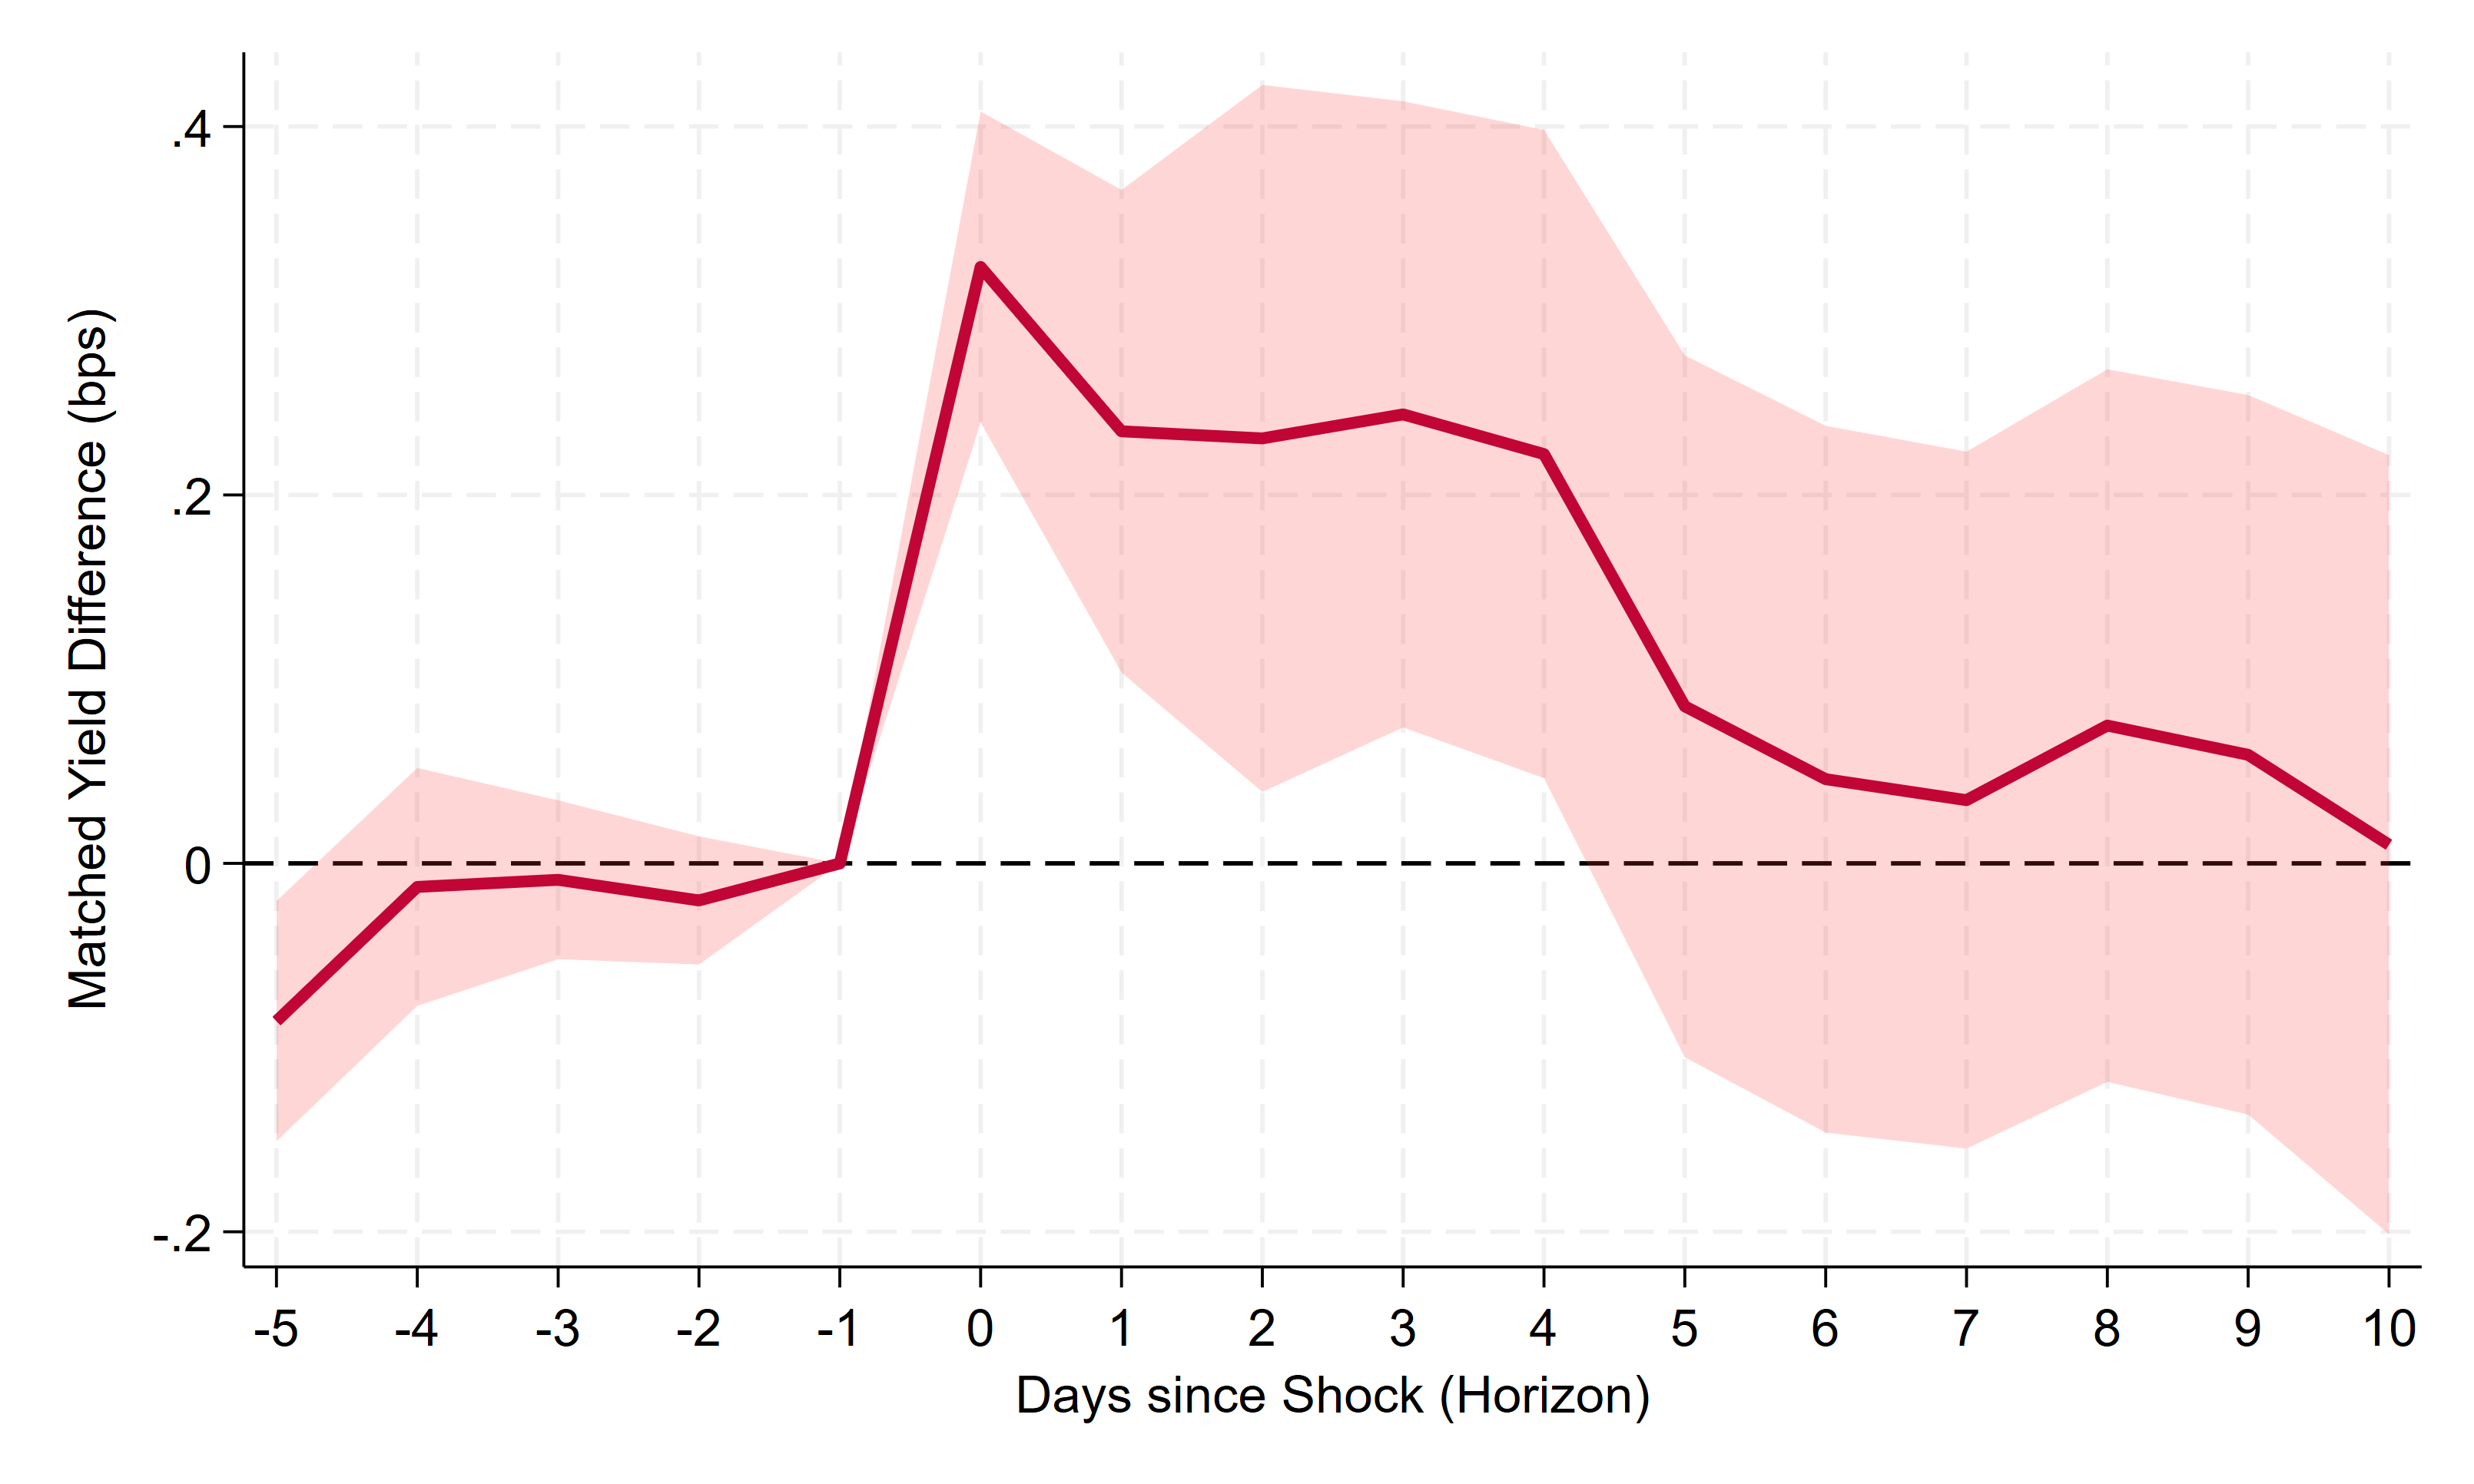
\includegraphics[width=\textwidth,height=0.5\textheight,keepaspectratio]{Figures/IR_baseline.png}}\\
{\scriptsize (a) Matched differential}
\end{column}
\begin{column}{0.5\textwidth}
\centering
\panR{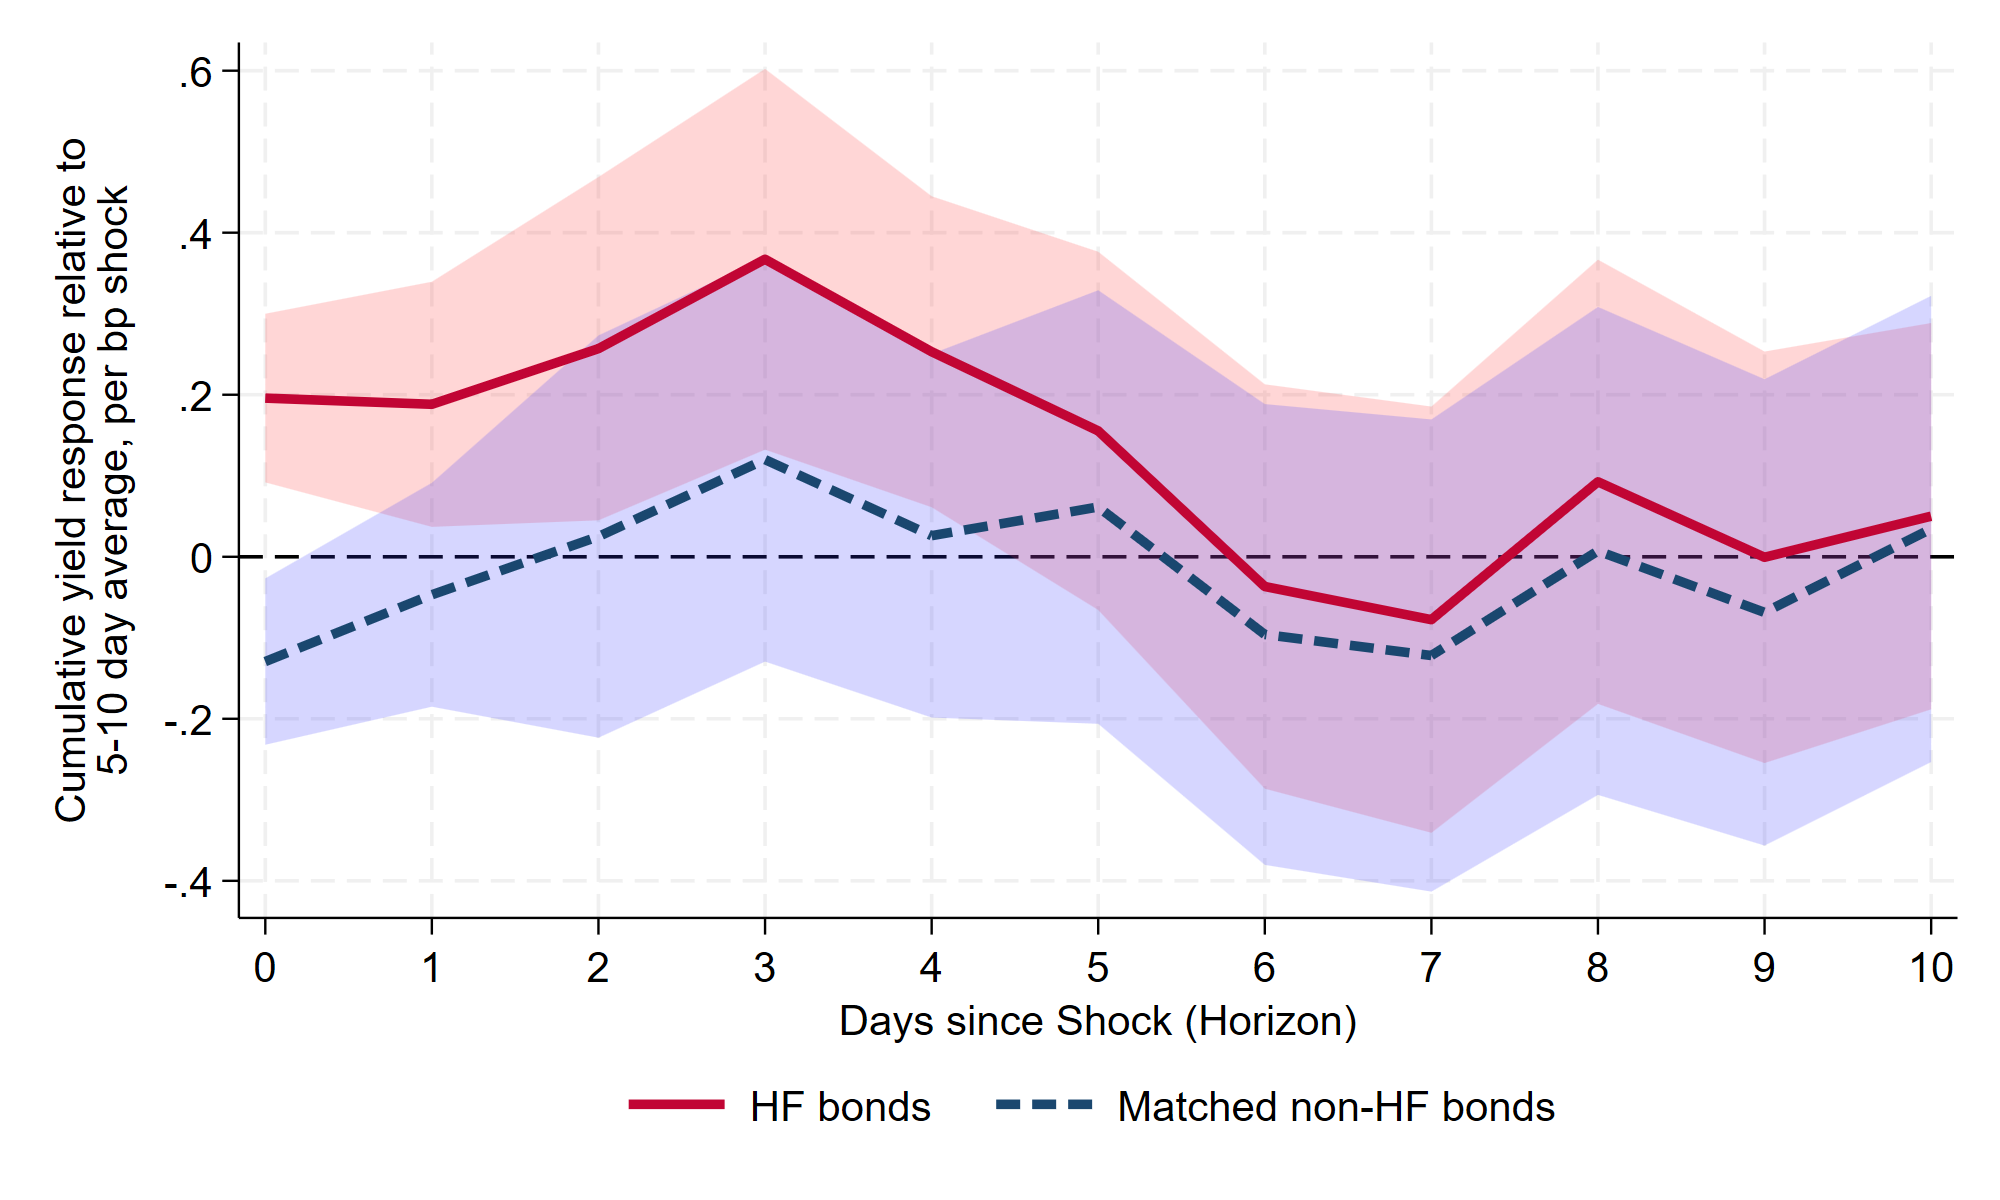
\includegraphics[width=\textwidth,height=0.5\textheight,keepaspectratio]{Figures/IR_baseline_decomposition_overshoot.png}}\\
{\scriptsize (b) Level decomposition}
\end{column}
\end{columns}
\twopanelnote{0.098}{0.979}{Local projections on the matched sample {\citep{jorda2005}}. Shaded areas are 90\% confidence intervals clustered by date and bond.}
\begin{columns}[t]
\begin{column}{0.5\textwidth}{\footnotesize Flat before the shock, immediate divergence on impact, significant for about \hibl{four days}, then reversion.}\end{column}
\begin{column}{0.5\textwidth}{\footnotesize Both legs converge to a common level. Hedge fund bonds \hird{overshoot} first.}\end{column}
\end{columns}
\takeaway{A temporary dislocation that other capital gradually absorbs, consistent with slow moving capital}
\navbtn{jkdecomp}{Not price discovery}
\end{frame}

% --- "The amplification is not price discovery" moved to the annex (linked from the overshoot slide) ---

% Verbal cues: within same dealer same day, only HF leg amplifies (0.271 to 0.250).
% Triple interaction with the dealer's own CDS change is ~0 -> not dealer stress.
\begin{frame}{The trigger is hedge fund positioning, not dealer behavior}
\vspace{0.2cm}
\begin{center}
\scriptsize
\setlength{\tabcolsep}{9pt}
\renewcommand{\arraystretch}{1.2}
\measurebox{\begin{tabular}{lcccc}
\toprule
\textbf{$\Delta$ yield (bps)} & (1) & (2) & (3) & (4) \\
\midrule
\rowcolor{goetheblue!8}
HF involved $\times$ Shock & 0.271$^{***}$ & 0.294$^{***}$ & 0.248$^{***}$ & 0.250$^{***}$ \\
HF involved (level)       & 0.006 & 0.007$^{*}$ & 0.001 & 0.001 \\
HF $\times$ Shock $\times$ $\Delta$CDS &  &  &  & 0.000 \\
\midrule
Bond controls             & Yes & Yes & Yes & Yes \\
Bond FE                       & Yes & Yes & Yes & Yes \\
Dealer $\times$ Date FE        & Yes & No & No & No \\
Dealer $\times$ Date $\times$ Country FE & No & Yes & No & No \\
Dealer $\times$ Date $\times$ Dur. FE & No & No & Yes & Yes \\
\bottomrule
\end{tabular}}
\end{center}
\fignote{Unit of observation is dealer, bond, day, balanced with zeros. $\Delta$CDS is the dealer's own five day CDS change before the shock. Standard errors clustered by dealer, date, and bond.}
Comparing bonds traded by the \hibl{same dealer on the same day}, the hedge fund bonds still react more. The effect does \hird{not} scale with the dealer's own credit stress.
\takeaway{Dealers intermediate the flow, but the trigger is the leveraged positioning of the funds}
\end{frame}

\resultdivider{2}{The amplification scales with the size of the position}

% Verbal cues: 0.164 to 0.167 stable; within-bond identification; direct effect zero.
% 6 bps x ln(1+3) x 0.164 ~ 1.36 bps. Bigger positions amplify more in the same bond.
\begin{frame}{The amplification scales with position size}
\vspace{0.2cm}
\begin{center}
\scriptsize
\setlength{\tabcolsep}{9pt}
\renewcommand{\arraystretch}{1.2}
\measurebox{\begin{tabular}{lcccc}
\toprule
\textbf{$\Delta$ yield (bps)} & (1) & (2) & (3) & (4) \\
\midrule
\rowcolor{goetheblue!8}
Log HF intensity $\times$ Shock & 0.166$^{***}$ & 0.165$^{***}$ & 0.167$^{***}$ & 0.164$^{***}$ \\
Shock                           & 0.811$^{***}$ & 0.811$^{***}$ &  &  \\
Log HF intensity (level)        & 0.008 & $-$0.020 & $-$0.009 & $-$0.011 \\
\midrule
Bond controls                   & No & Yes & Yes & Yes \\
Bond FE                          & No & No & Yes & Yes \\
Date FE                          & No & No & Yes & No \\
Dur. $\times$ Date $\times$ Country FE & No & No & No & Yes \\
\bottomrule
\end{tabular}}
\end{center}
\fignote{Log HF intensity is the log of one plus the five day net position scaled by amount outstanding. Standard errors clustered by date and bond. $^{***}\,p<0.01$.}
Within the \hibl{same bond} over time, a larger position produces a larger reaction, which pure selection cannot explain. At a 6 bps shock and 3\% intensity this adds about \hibl{1.36 bps}.
\takeaway{A continuous dose response that complements the matched sample evidence}
\end{frame}

\resultdivider{3}{The amplification is symmetric across regimes}

% Verbal cues: constraining 0.140, relaxing 0.224, Wald p=0.16 (not distinguishable).
\begin{frame}{The amplification holds whether shocks help or hurt the position}
\lvs
\begin{columns}[c]
\begin{column}{0.46\textwidth}
\centering
\scriptsize
\setlength{\tabcolsep}{9pt}
\renewcommand{\arraystretch}{1.25}
\measurebox{\begin{tabular}{lcc}
\toprule
\textbf{$\Delta$ yield (bps)} & Constraining & Relaxing \\
\midrule
\rowcolor{goetheblue!8}
Log HF int. $\times$ Shock & 0.140$^{***}$ & 0.224$^{***}$ \\
Log HF int. (level)         & $-$0.016 & $-$0.009 \\
\midrule
Bond controls               & Yes & Yes \\
Bond FE & Yes & Yes \\
Dur.$\times$Date$\times$Ctry FE & Yes & Yes \\
\bottomrule
\end{tabular}}
\par\smallskip
\fignote{Each regime also includes all non shock days and zero intensity days as the within bond baseline. Standard errors clustered by date and bond.}
\end{column}
\begin{column}{0.5\textwidth}
\begin{wideitemize}
  \item \hird{Constraining} when the shock moves against the position
  \item \higr{Relaxing} when it moves in favor
  \item A Wald test \hibl{cannot distinguish} the two ($p=0.16$)
\end{wideitemize}
\end{column}
\end{columns}
\lvs
\begin{center}
\begin{tikzpicture}\node[keybox, text width=0.82\textwidth]{Comparable amplification in both states, which is what \emph{rebalancing toward a target} predicts};\end{tikzpicture}
\end{center}
\takeaway{Amplification is not only a crisis phenomenon, it operates whenever shocks meet positions}
\end{frame}

% Verbal cues: constraining contracts, relaxing expands; near symmetric -> constant
% leverage targeting. Both push yields in the direction of the shock.
\begin{frame}{Positions contract and expand as the mechanism predicts}
\hypertarget{positions}{}
\begin{center}
\measureplot{0.078}{0.973}{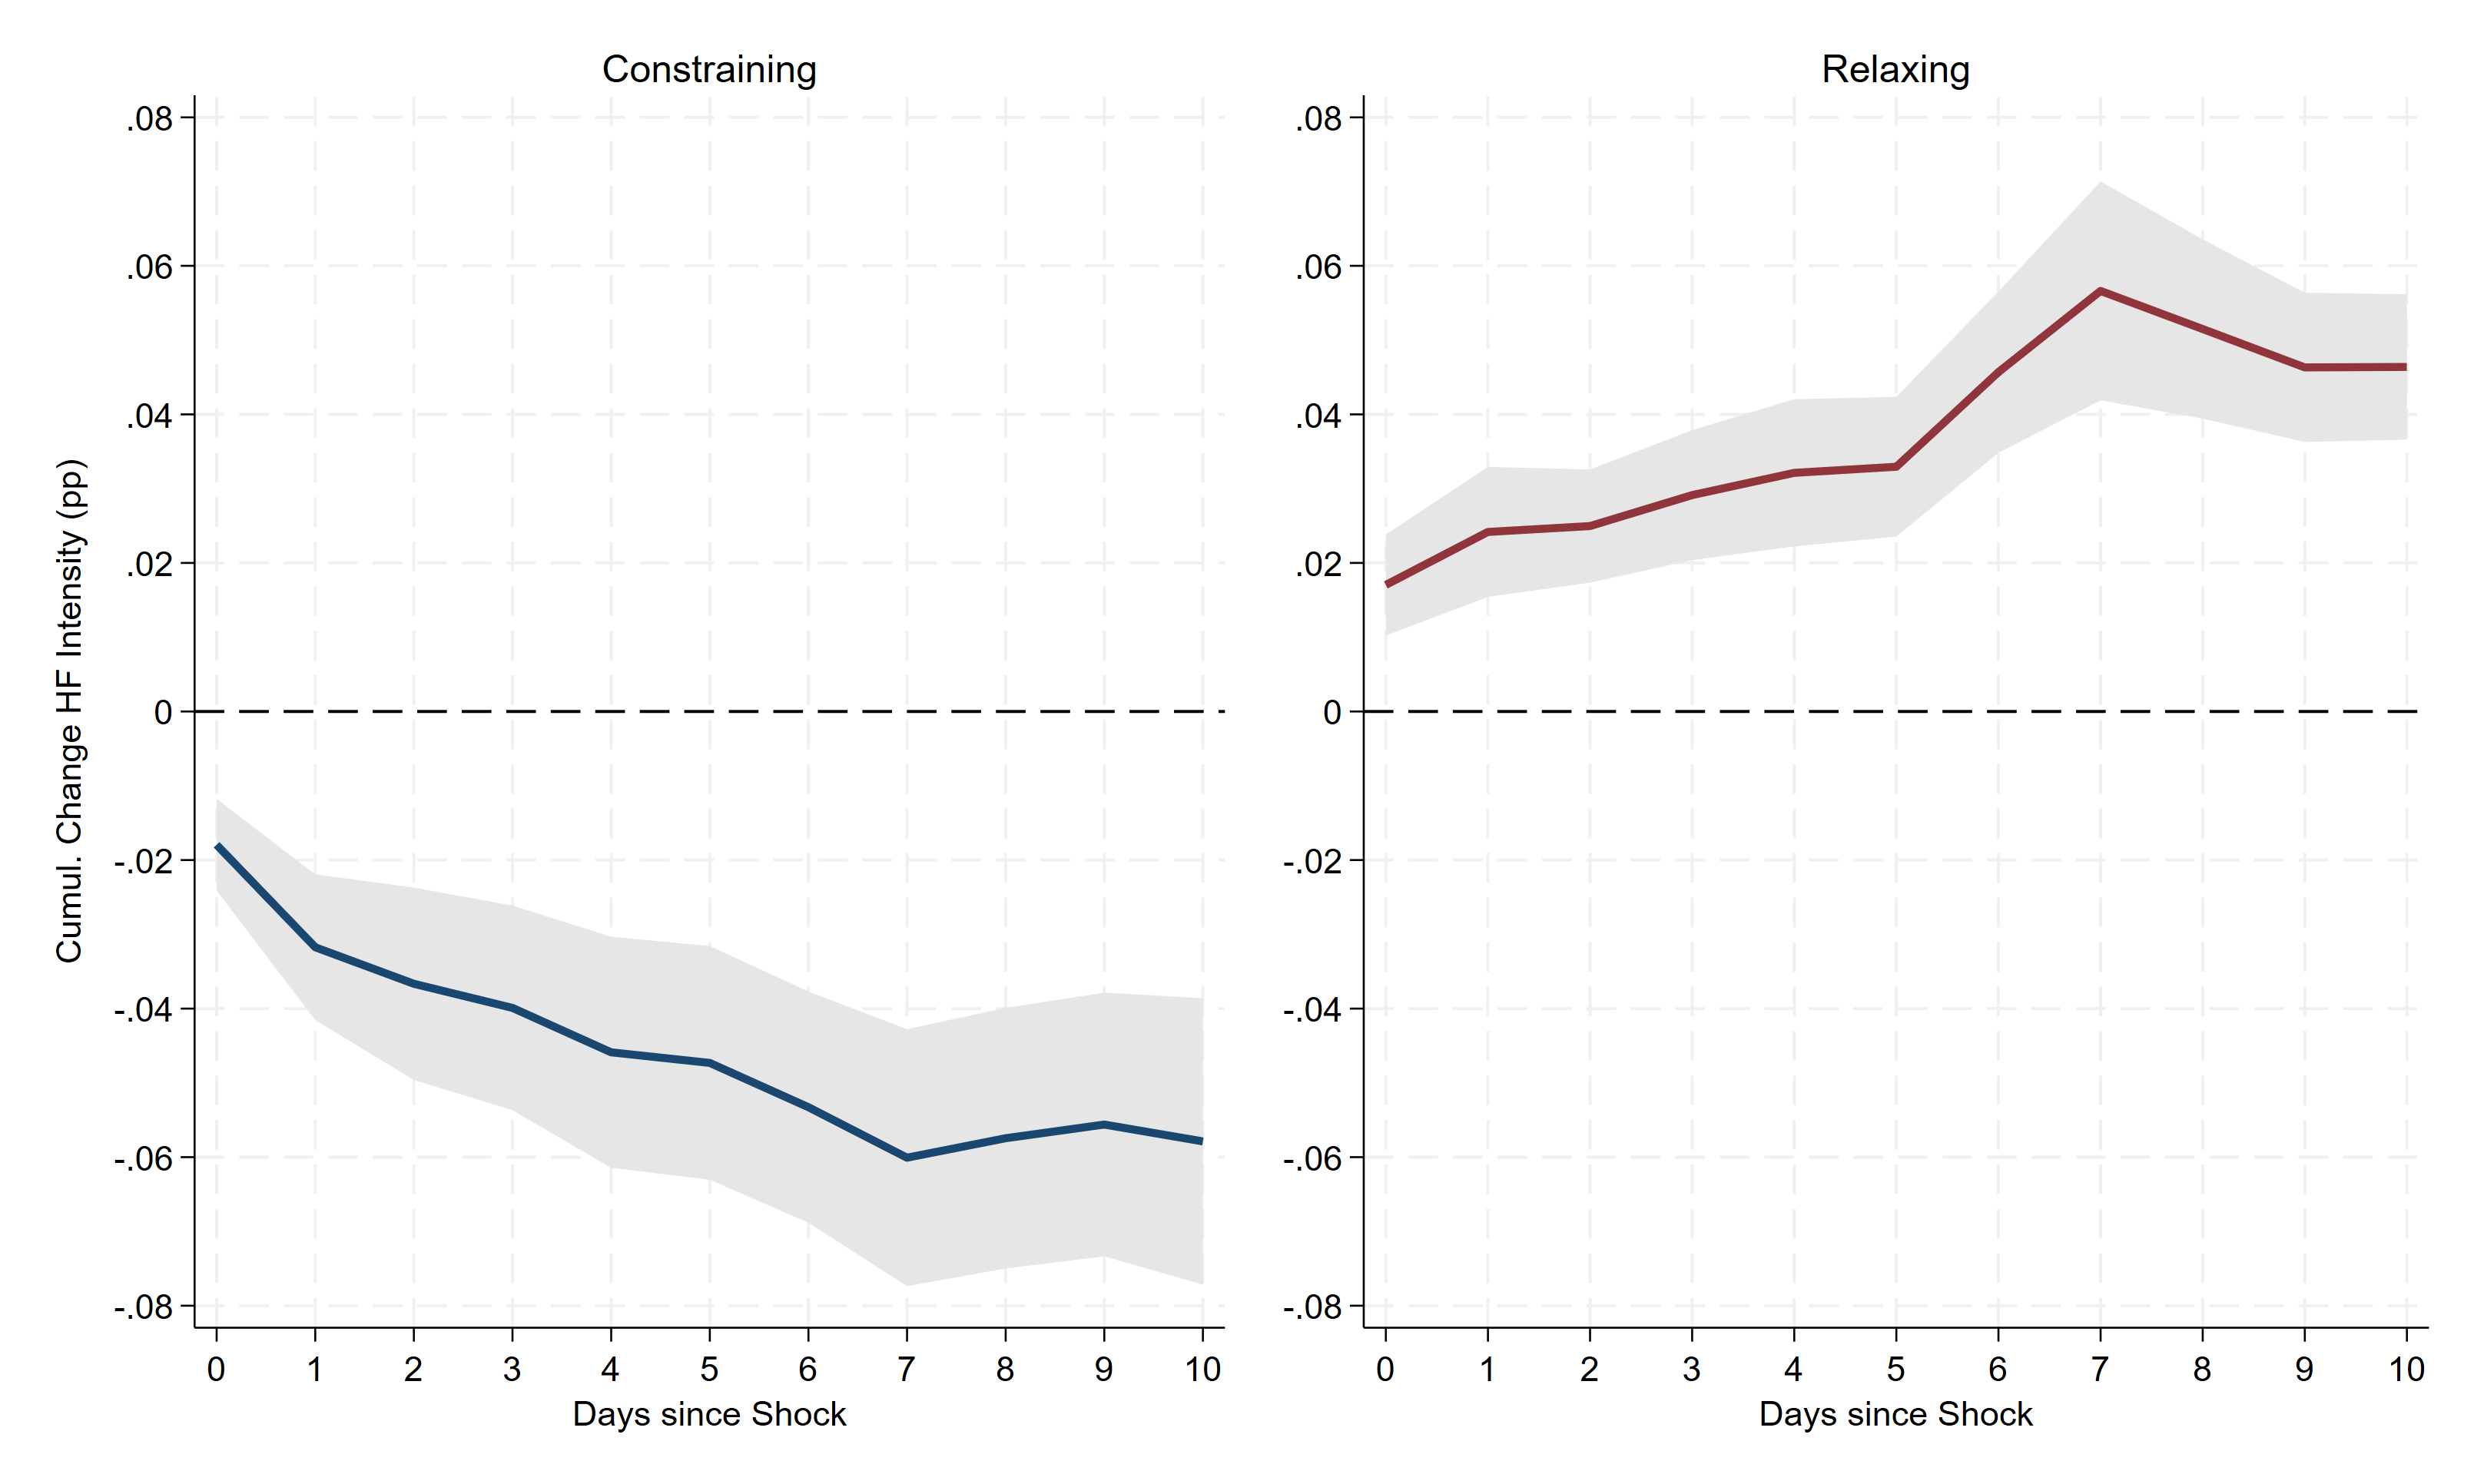
\includegraphics[height=0.56\textheight,keepaspectratio]{Figures/IR_on_momentum.png}}
\end{center}
\fignote{Cumulative change in hedge fund intensity from $t-1$ to $t+h$ after a shock, by regime, local projections on overnight repo {\citep{jorda2005}}. Bond and duration $\times$ country $\times$ date fixed effects. Shaded areas are 90\% confidence intervals. Sample period 2021 to 2025.}
\takeaway{Funds reduce exposure in the constraining state and add in the relaxing state, the signature of constant leverage targeting}
\navbtn{termrepo}{Term repo}
\end{frame}

\resultdivider{4}{The directionality of the book governs the strength}

\begin{frame}{Book directionality, not only size}
\lvs
\lead{The constraint binds at the level of the whole book}
\bit
  \item A book long Italy and short Germany of similar duration carries little net exposure to a parallel rate move, so a shock barely moves its capital
  \item A one sided directional book absorbs the full loss and rebalances
\eit
\lvs
\lead{A bond level measure of holder directionality}
\beq
\text{Dir}_{f,t}=\frac{\left|\sum_i D_i\,q_{f,i,t}\right|}{\sum_i D_i\,|q_{f,i,t}|},
\qquad
\text{HolderDir}_{i,t}=\frac{\sum_f |q_{f,i,t}|\,\text{Dir}_{f,t}}{\sum_f |q_{f,i,t}|}
\eeq
\svs
{\footnotesize Zero when long and short legs offset in duration, close to one when the book is one sided. Each bond inherits the position weighted directionality of the funds holding it.}
\takeaway{A more hedged book behaves like a higher effective margin in the mechanism}
\end{frame}

\begin{frame}{The sector rotates between hedged and directional books}
\begin{center}
\measureplot{0.099}{0.982}{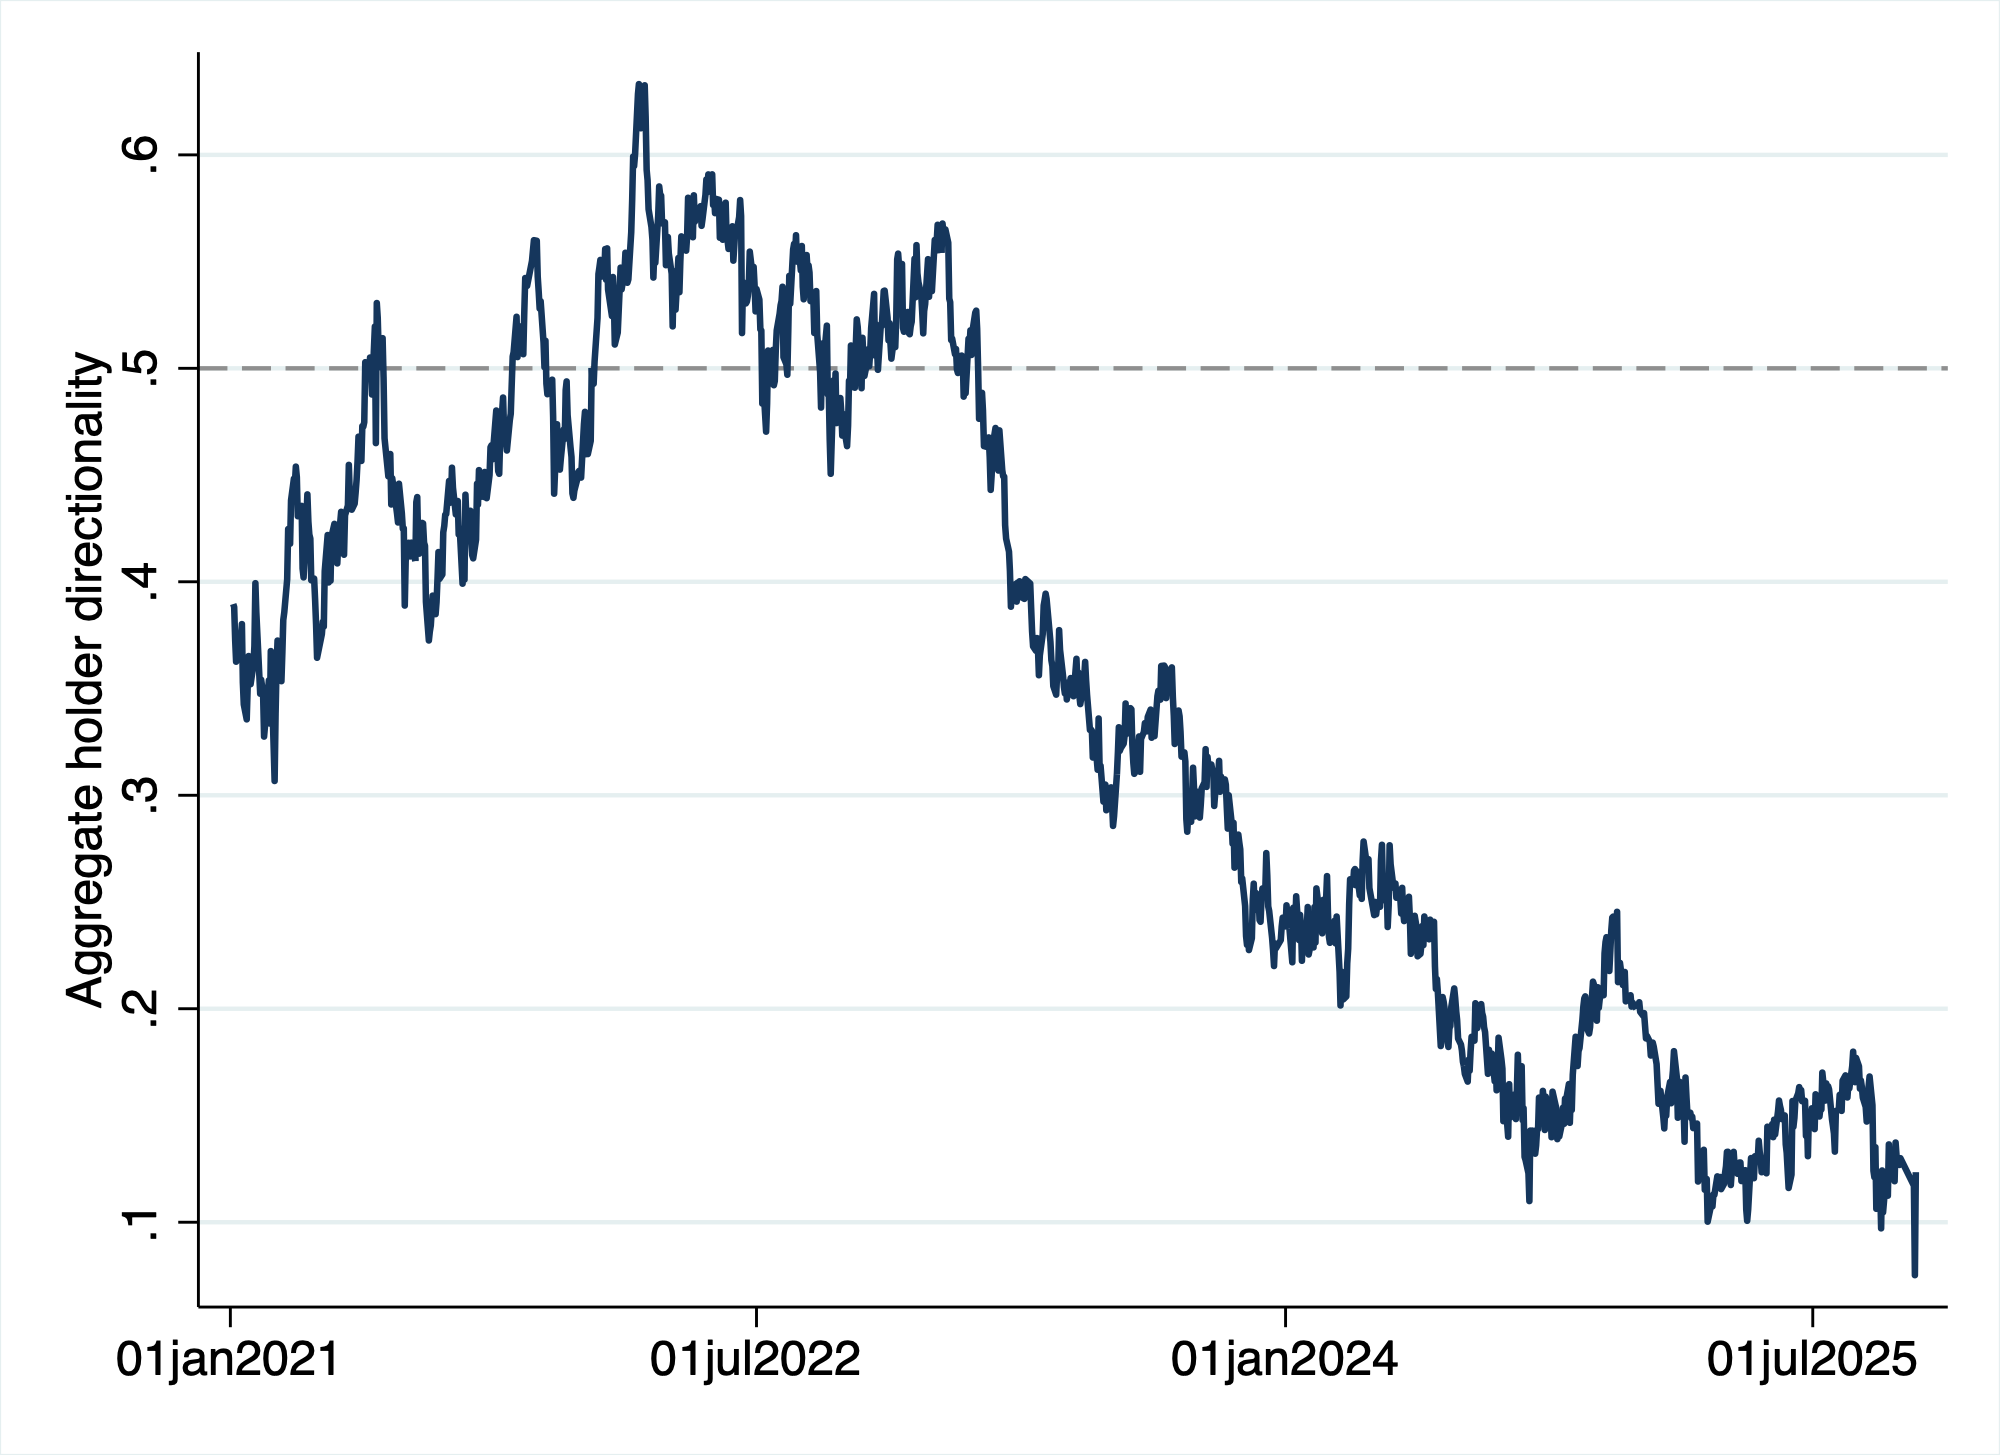
\includegraphics[height=0.56\textheight,keepaspectratio]{Figures/holder_dir_timeseries.png}}
\end{center}
\fignote{Position weighted average of holder directionality across bonds. High when bonds are held mainly within directional books. Within duration, country, and date cells the average dispersion is about 0.11, which is the variation that identifies the next result. Sample period 2021 to 2025.}
\takeaway{Directional through the hiking cycle, then back toward hedged relative value in 2024 and 2025}
\end{frame}

% Verbal cues: hedged 0.098, directional 0.363, F=24.8; quartiles rise monotonically
% 0.057 -> 0.367. Within-cell FE absorbs the common monetary environment.
\begin{frame}{Amplification is concentrated in directional books}
\vspace{0.2cm}
\begin{center}
\scriptsize
\setlength{\tabcolsep}{12pt}
\renewcommand{\arraystretch}{1.2}
\measurebox{\begin{tabular}{lc}
\toprule
\textbf{$\Delta$ yield (bps), relative to no HF} & Coefficient \\
\midrule
Hedged book $\times$ Shock        & 0.098$^{***}$ \\
\rowcolor{goetheblue!8}
Directional book $\times$ Shock   & 0.363$^{***}$ \\
\midrule
\multicolumn{2}{l}{\textit{By directionality quartile}}\\
Q1 most hedged $\times$ Shock      & 0.057 \\
Q2 $\times$ Shock                  & 0.137$^{***}$ \\
Q3 $\times$ Shock                  & 0.361$^{***}$ \\
\rowcolor{goetheblue!8}
Q4 most directional $\times$ Shock & 0.367$^{***}$ \\
\midrule
Bond controls                      & Yes \\
Bond FE                            & Yes \\
Dur. $\times$ Date $\times$ Country FE & Yes \\
\bottomrule
\end{tabular}}
\end{center}
\fignote{Bond and duration $\times$ country $\times$ date fixed effects with controls. Wald tests reject equality of the hedged and directional groups ($F=24.8$) and of the extreme quartiles ($F=28.3$). Standard errors clustered by date and bond.}
The amplification rises \hibl{monotonically} with directionality and is \hird{not distinguishable from zero} in the most hedged quartile.
\takeaway{Same shock, same day, same maturity and country, the directional holders carry the effect}
\end{frame}


%========================================================================================
\sectionframe{Conclusion}
%========================================================================================

% --- Robustness is shown as four individual annex slides (expanded sample, credit shock,
%     volatility standardized, placebo); reachable via the Robustness button on the conclusion. ---

\begin{frame}{Conclusion}
\hypertarget{conclusion}{}
\lvs
\lead{What the paper shows}
\ben\itemsep4pt
  \item Hedge fund trading amplifies yield sensitivity, more than a quarter of the shock day move
  \item The effect scales with position size and reverts within days, a temporary overshoot
  \item It is symmetric across the constraining and relaxing states, consistent with constant leverage targeting
  \item It is concentrated in \hird{directional} books and close to zero in \hibl{hedged} books
\een
\lvs
\lead{For risk monitoring}
\bit\itemsep3pt
  \item Size and presence alone are not sufficient, and amplification is not confined to stress episodes
  \item The \hird{directionality} of the book is a key risk metric beyond position size
\eit
\vfill
\begin{center}{\color{goetheblue}\textbf{Thank you}}\end{center}
\vfill
\navbtn{extval}{Robustness}
\end{frame}

%========================================================================================
% References
%========================================================================================
\begin{frame}[allowframebreaks]{References}
\tiny
\printbibliography[heading=none]
\end{frame}

%========================================================================================
\sectionframe{Annex}
%========================================================================================
\appendix

% --- Summary statistics (linked from the footprint slide) ---
\begin{frame}{Summary statistics}
\hypertarget{summ_full}{}
\begin{center}
\scriptsize
\setlength{\tabcolsep}{5pt}
\renewcommand{\arraystretch}{1.12}
\measurebox{\begin{tabular}{lcccccc}
\toprule
 & Mean & SD & P25 & Median & P75 & N \\
\midrule
\multicolumn{7}{l}{\textit{Bond market}}\\
Daily yield change (bps) & 0.15 & 5.79 & $-2.25$ & 0.00 & 2.75 & 477{,}001 \\
Duration (years)         & 7.13 & 7.00 & 1.77 & 5.14 & 10.47 & 477{,}001 \\
Bid ask spread (\euro)   & 0.31 & 0.42 & 0.03 & 0.11 & 0.44 & 477{,}001 \\
\addlinespace
\multicolumn{7}{l}{\textit{Hedge fund positioning}}\\
HF present (dummy)       & 0.53 & 0.50 & 0.00 & 1.00 & 1.00 & 477{,}001 \\
Net position, active (\% issued) & 3.01 & 3.29 & 0.64 & 1.80 & 4.26 & 253{,}111 \\
\addlinespace
\multicolumn{7}{l}{\textit{Repo terms, active}}\\
Haircut, long (\%)       & 0.24 & 0.54 & 0.00 & 0.12 & 0.30 & 109{,}068 \\
Maturity, long (days)    & 16.49 & 16.42 & 7.50 & 11.00 & 18.65 & 101{,}535 \\
\addlinespace
\multicolumn{7}{l}{\textit{Shock days}}\\
Tightening surprise (bps) & 5.87 & 4.10 & 3.30 & 4.95 & 7.60 & 5{,}736 \\
Easing surprise (bps)     & $-4.17$ & 4.48 & $-6.72$ & $-3.13$ & $-0.56$ & 8{,}803 \\
\bottomrule
\end{tabular}}
\end{center}
\fignote{Daily panel of German and Italian sovereign bonds. Positioning variables are five day moving averages scaled by amount outstanding. Sample period 2021 to 2025.}
\navbtn{footprint}{Back}
\end{frame}

% --- Why these shocks (exceedance) ---
\begin{frame}{Monetary surprises generate fat tails in yield changes}
\hypertarget{exceedance}{}
\begin{center}
\measureplot{0.064}{0.981}{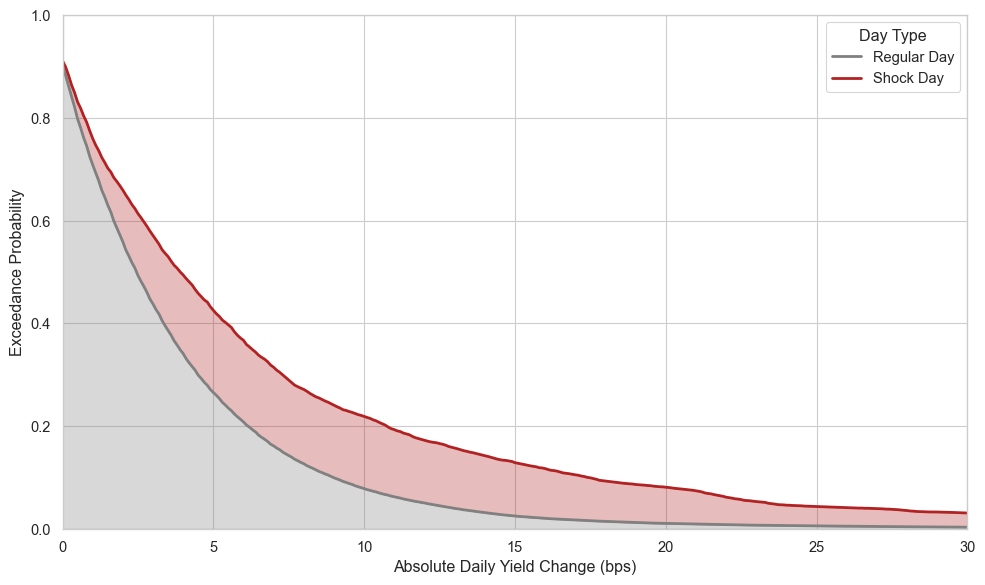
\includegraphics[width=0.6\textwidth]{Figures/exceedance_probability.png}}
\end{center}
\fignote{Share of bond days where the absolute yield change exceeds the threshold on the horizontal axis. Red is monetary announcement days, grey is regular days. The gap is the excess tail risk from surprises. Sample period 2021 to 2025.}
\takeaway{Surprises move yields enough to activate the mechanism}
\navbtn{specification}{Back}
\end{frame}

% --- Not price discovery (moved from main body; linked from the overshoot slide) ---
\begin{frame}{The amplification is not price discovery}
\hypertarget{jkdecomp}{}
\lvs
A price discovery story predicts \hibl{stronger} amplification when the surprise carries new fundamental information.
\svs
\begin{center}
\scriptsize
\setlength{\tabcolsep}{16pt}
\renewcommand{\arraystretch}{1.25}
\measurebox{\begin{tabular}{lcc}
\toprule
\textbf{$\Delta$ yield (bps)} & (1) Pure monetary & (2) Information \\
\midrule
\rowcolor{goetheblue!8}
HF involved $\times$ Shock & 0.377$^{***}$ & 0.113$^{***}$ \\
HF involved (level)        & $-$0.019 & $-$0.026 \\
\midrule
Bond controls              & Yes & Yes \\
Bond FE                    & Yes & Yes \\
Dur. $\times$ Date $\times$ Country FE & Yes & Yes \\
\bottomrule
\end{tabular}}
\end{center}
\fignote{Both columns include bond and duration $\times$ country $\times$ date fixed effects and controls. A Wald test rejects equality ($p=0.065$). Standard errors clustered by date and bond.}
The amplification is concentrated in the \hird{pure monetary} component, the part that carries \hird{no} new fundamental information. This is the \hibl{opposite} of the price discovery prediction.
\takeaway{Decomposing the surprise points the same way as the overshooting {\scriptsize\citep{jarocinski2020}}}
\navbtn{overshoot}{Back}
\end{frame}

% --- Term repo IR (linked from the positions-contract slide) ---
\begin{frame}{Term repo shows the same pattern with a lag}
\hypertarget{termrepo}{}
\begin{center}
\measureplot{0.078}{0.973}{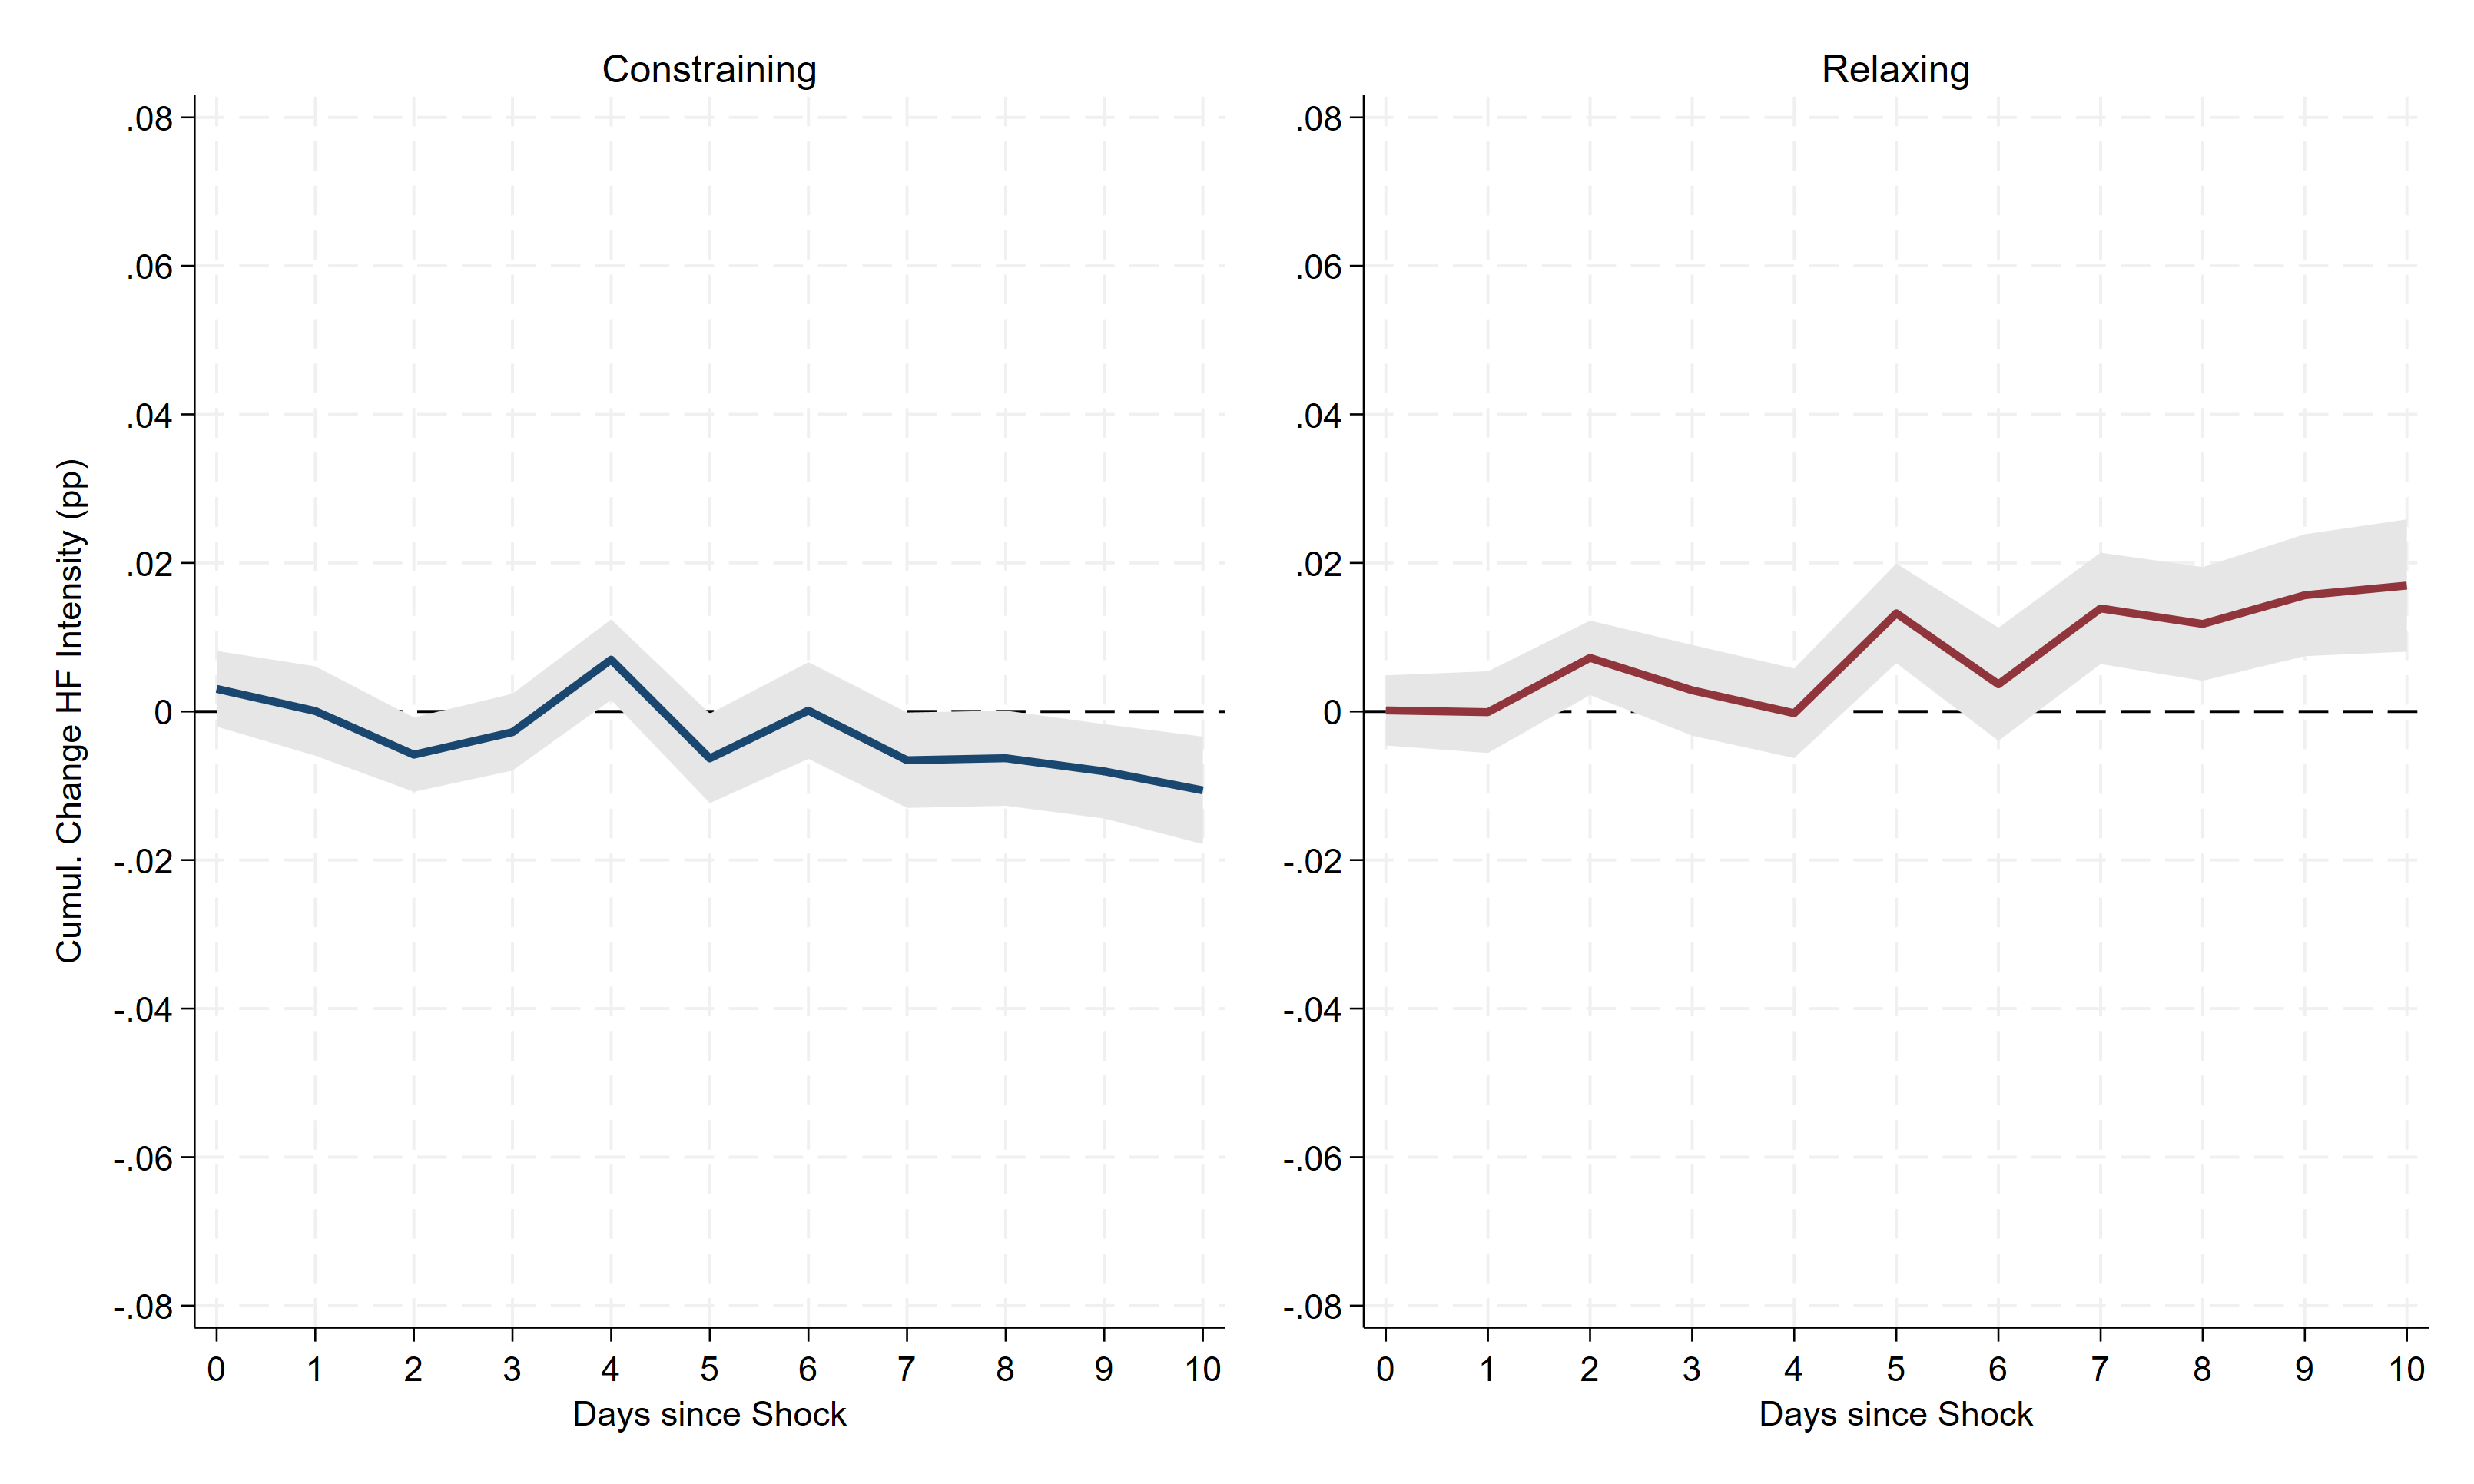
\includegraphics[width=0.6\textwidth]{Figures/IR_term_momentum.png}}
\end{center}
\fignote{Cumulative change in hedge fund intensity by regime, term repo only, local projections \citep{jorda2005}. Same contraction and expansion as overnight, delayed by about five days in line with the maturity profile. Sample period 2021 to 2025.}
\navbtn{positions}{Back}
\end{frame}

% --- External validity table ---
\begin{frame}{External validity, expanded sovereign sample}
\hypertarget{extval}{}
\begin{center}
\scriptsize
\setlength{\tabcolsep}{9pt}
\renewcommand{\arraystretch}{1.2}
\measurebox{\begin{tabular}{lcccc}
\toprule
\textbf{$\Delta$ yield (bps)} & (1) Presence & (2) Intensity & (3) Constraining & (4) Relaxing \\
\midrule
\rowcolor{goetheblue!8}
HF involved $\times$ Shock      & 0.192$^{***}$ &  &  &  \\
\rowcolor{goetheblue!8}
Log HF intensity $\times$ Shock &  & 0.122$^{***}$ & 0.107$^{***}$ & 0.171$^{***}$ \\
HF involved (level)             & $-$0.046 &  &  &  \\
Log HF intensity (level)        &  & $-$0.015 & $-$0.019 & $-$0.012 \\
\midrule
Bond controls                   & Yes & Yes & Yes & Yes \\
Bond FE                          & Yes & Yes & Yes & Yes \\
Dur. $\times$ Date $\times$ Country FE & Yes & Yes & Yes & Yes \\
\bottomrule
\end{tabular}}
\end{center}
\fignote{Adds French and Spanish sovereigns to the German and Italian baseline. Bond and duration $\times$ country $\times$ date fixed effects with controls. Standard errors clustered by date and bond. $^{***}\,p<0.01$.}
Germany, Italy, France, and Spain. All coefficients stay positive and significant, somewhat smaller, consistent with hedge funds being less active in French and Spanish bonds.
\navbtn{baseline}{Back}
\end{frame}

% --- Credit shock robustness ---
\begin{frame}{Amplification under a sovereign credit shock}
\begin{center}
\scriptsize
\setlength{\tabcolsep}{9pt}
\renewcommand{\arraystretch}{1.2}
\measurebox{\begin{tabular}{lcccc}
\toprule
\textbf{$\Delta$ yield (bps)} & (1) & (2) & (3) Constraining & (4) Relaxing \\
\midrule
\rowcolor{goetheblue!8}
HF involved $\times$ Shock      & 0.225$^{***}$ &  &  &  \\
\rowcolor{goetheblue!8}
Log HF intensity $\times$ Shock &  & 0.107$^{***}$ & 0.129$^{***}$ & 0.117$^{***}$ \\
HF involved (level)             & $-$0.030 &  &  &  \\
Log HF intensity (level)        &  & $-$0.021 & $-$0.022 & $-$0.020 \\
\midrule
Bond controls                   & Yes & Yes & Yes & Yes \\
Bond FE                          & Yes & Yes & Yes & Yes \\
Dur. $\times$ Date $\times$ Country FE & Yes & Yes & Yes & Yes \\
\bottomrule
\end{tabular}}
\end{center}
\fignote{Standard errors clustered by date and bond. $^{***}\,p<0.01$.}
The shock is the residual of the daily change in the five year US dollar Italian sovereign CDS spread, restricted to its 2\% tails, away from ECB events. The two regimes are close in magnitude.
\end{frame}

% --- Volatility-standardized robustness ---
\begin{frame}{Volatility standardized yield changes}
\begin{center}
\scriptsize
\setlength{\tabcolsep}{9pt}
\renewcommand{\arraystretch}{1.2}
\measurebox{\begin{tabular}{lcccc}
\toprule
\textbf{Standardized $\Delta$ yield ($\sigma$ units)} & (1) & (2) & (3) Constraining & (4) Relaxing \\
\midrule
\rowcolor{goetheblue!8}
HF involved $\times$ Shock      & 0.043$^{***}$ &  &  &  \\
\rowcolor{goetheblue!8}
Log HF intensity $\times$ Shock &  & 0.020$^{***}$ & 0.016$^{***}$ & 0.031$^{***}$ \\
HF involved (level)             & $-$0.007 &  &  &  \\
Log HF intensity (level)        &  & $-$0.004 & $-$0.005 & $-$0.004 \\
\midrule
Bond controls                   & Yes & Yes & Yes & Yes \\
Bond FE                          & Yes & Yes & Yes & Yes \\
Dur. $\times$ Date $\times$ Country FE & Yes & Yes & Yes & Yes \\
\bottomrule
\end{tabular}}
\end{center}
\fignote{Standard errors clustered by date and bond. $^{***}\,p<0.01$.}
Each yield change is divided by the bond's own conditional volatility from a GARCH(1,1) fit on non shock days. With average $\hat\sigma$ near 6 bps these map back to roughly 0.26 and 0.12 bps per bp, close to the baseline.
\end{frame}

% --- Placebo (shifted shock dates) ---
\begin{frame}{Placebo with shifted shock dates}
\begin{center}
\scriptsize
\setlength{\tabcolsep}{9pt}
\renewcommand{\arraystretch}{1.2}
\measurebox{\begin{tabular}{lcccc}
\toprule
\textbf{$\Delta$ yield (bps)} & (1) & (2) & (3) Constraining & (4) Relaxing \\
\midrule
\rowcolor{goetheblue!8}
HF involved $\times$ Placebo shock      & $-$0.030 &  &  &  \\
\rowcolor{goetheblue!8}
Log HF intensity $\times$ Placebo shock &  & $-$0.018 & $-$0.014 & $-$0.028 \\
Placebo shock                           & 0.007 & 0.004 & 0.002 & $-$0.003 \\
HF involved (level)                     & $-$0.031 &  &  &  \\
Log HF intensity (level)                &  & $-$0.018 & $-$0.017 & $-$0.020 \\
\midrule
Bond controls                           & Yes & Yes & Yes & Yes \\
Bond FE                                  & Yes & Yes & Yes & Yes \\
Dur. $\times$ Date $\times$ Country FE  & Yes & Yes & Yes & Yes \\
\bottomrule
\end{tabular}}
\end{center}
\fignote{Monetary shock dates shifted by 15 trading days, which breaks the timing. Standard errors clustered by date and bond.}
Shifting the shock dates removes the coincidence with announcements. The amplification disappears entirely, which ties it to the actual shock.
\end{frame}

\end{document}
